\documentclass[times, 10pt]{article} 
%\documentclass[times, 10pt,twocolumn]{article} 
%\usepackage[noend]{distribalgo}
\usepackage{algorithm}
%\usepackage{times}
\usepackage{amsmath}
\usepackage{amsthm}
\usepackage{graphicx}
\usepackage{color}
\usepackage{amssymb}
\usepackage[noend]{distribalgo}
\usepackage[draft]{fixme}
\usepackage[hmargin=2.5cm,vmargin=2.2cm]{geometry}


\begin{document}

\newcommand{\mv}[1]{\ensuremath{\operatorname{\mathit{#1}}}}
\definecolor{dark}{gray}{.6}
\newcommand{\bc}[1]{\textcolor{dark}{#1}}
\newtheorem{lems}{Lemma}
\newtheorem{props}{Proposition}
\newtheorem{thms}{Theorem}
\newtheorem{defs}{Definition}
\newtheorem{obs}{Observation}

\newcommand{\code}[1]{\texttt{\small{\textbf{#1}}}}

\newcommand{\blankline}{\vspace{4 mm}}
\newcommand{\amcast}{\mbox{multicast}}
\newcommand{\amdel}{\mbox{deliver}}
\newcommand{\amdelarg}[1]{\mbox{\amdel({#1})}}
\newcommand{\amcastarg}[1]{\mbox{\amcast({#1})}}
\newcommand{\tconsm}{T_{cons}}
\newcommand{\tcons}{\mbox{$\tconsm$}}
\newcommand{\optdel}{\mbox{opt-deliver}}
\newcommand{\consdel}{\amdel}
\newcommand{\rmcast}{\mbox{fr-mcast}}
\newcommand{\rmdel}{\mbox{fr-deliver}}
\newcommand{\optdelarg}[1]{\mbox{\opt({#1})}}
\newcommand{\consdelarg}[1]{\amdelarg{#1}}
\newcommand{\rmcastarg}[2]{\mbox{\rmcast({#1},{#2})}}
\newcommand{\rmdelarg}[1]{\mbox{\rmdel({#1})}}

\newcommand{\localmsgs}{messages\text{$_g$}}
\newcommand{\decided}{decided\text{$_g$}}
\newcommand{\stamped}{stamped}
\newcommand{\delivered}{delivered}%{a\mbox{-}delivered}2

%\NewDocumentCommand \mycast { g }
%{\IfNoValueTF{#1}{\amcast}{\amcastarg{#1}}}

%\title{Optimistic Atomic Multicast}
\title{Optimistic Atomic Multicast in One Communication Delay}
%\title{A Quasi-Genuine Fifo Total Order Multicast Primitive}

%\author{
%xxx\\
%University \\ Country\\
%\and
%xxx\\
%University \\ Country\\
%\and
% ...
%}

\maketitle

\begin{abstract}

\end{abstract}

\section{Introduction}
\label{sec:intro}

Some multicast primitives have been devised in such a way that multicast groups needed to communicate only when they had messages to exchange. These multicast primitives are called \emph{genuine}. We argue that it is possible, however, to devise a multicast primitive that, although not genuine, can make use of some knowledge given by the application to figure out which groups \emph{can} communicate with each other. With such knowledge, although message exchanges take place even when there is no application message being transmitted between some two groups, such exchanges happen only when they are able to send to -- or receive from -- one another. The primitive that makes use of such property we call \emph{quasi-genuine}. 

\section{System model and definitions}
\label{sec:model}

In this section we introduce the underlying system model and define two higher-level abstractions: consensus and atomic multicast. As we discuss later in the paper, atomic multicast builds on the consensus abstraction.

\subsection{Processes and communication}

We consider a system $\Pi = \{ p_1, ..., p_n \}$ of processes which communicate through message passing and do not have access to a shared memory or a global clock. The system is asynchronous: messages may experience arbitrarily large (but finite) delays and there is no bound on relative process speeds. We assume the benign crash-stop failure model: processes may fail by crashing, but do not behave maliciously. A process that never crashes is \emph{correct}; otherwise it is \emph{faulty}. We define $\Gamma = \{ g_1, ..., g_m \}$ as the set of process groups in the system. Groups are disjoint, non-empty, and satisfy $\bigcup_{g \in \Gamma} g = \Pi$. For each process $p \in \Pi$, $group(p)$ identifies the group $p$ belongs to. For the sake of simplicity, we abuse the notation by writing ``$p \in \gamma$'', instead of ``$\exists g \in \gamma: p \in g$'', where $\gamma$ is any set of groups, such that $\gamma \subseteq \Gamma$. Hereafter, we assume that each group can solve consensus, a problem we define next.

Processes communicate using fifo reliable multicast, defined by the primitives \rmcast{}$(s,m)$ and \rmdel{}$(m)$, where $s$ is a set of groups and $m$ is a message. Reliable multicast guarantees that (i)~for any process $p$ and any message $m$, $p$ \rmdel{}s $m$ at most once, and only if $p \in s$ and $m$ was previously \rmcast{} \emph{(uniform integrity)}; (ii)~if a correct process $p$ \rmcast{}s $m$, then eventually all correct processes $q \in s$ \rmdel{} $m$ \emph{(validity)}; (iii)~if $p$ \rmdel{}s $m$, then eventually all correct processes $q \in s$ \rmdel{}s $m$ \emph{(uniform agreement)}; and (iv)~if $p$ \rmcast{}s $m$ and then $m'$, then no $q$ \rmdel{}s $m'$ without first \rmdel{}ing $m$ \emph{(fifo order)}.


\subsection{Consensus}

An important part of this work relies on the use of consensus to ensure that processes agree upon which messages are delivered and in which order they are delivered. We consider instances of consensus solved within a group. Moreover, we distinguish multiple instances of consensus executed within the same group with unique natural numbers.
Consensus is defined by the primitives \textit{propose$_g(k, v)$} and \textit{decide$_g(k, v)$}, where $g$ is a group, $k$ a natural number and $v$ a value, and satisfies the following properties in each instance $k$~\cite{hadzilacos1993ftb}:
(i)~if process $p \in g$ decides $v$, then $v$ was previously proposed by some process in $g$ \emph{(uniform integrity)}; 
(ii)~if $p \in g$ decides $v$, then all correct processes in $g$ eventually decide $v$ \emph{(uniform agreement)}; and 
(iii)~every correct process in $g$ eventually decides exactly one value \emph{(termination)}.


\subsection{Atomic multicast}

Atomic multicast ensures that messages can be addressed to a set of groups. %For any message $m$, $m.dst$ denotes the groups to which $m$ is atomically multicast. By abuse of notation, we write process ``$p \in m.dst$" instead of ``$\exists g \in m.dst$ such that $p \in g$". 
Atomic multicast is defined by the primitives \amcastarg{$(m)$} and \amdelarg{$(m)$}, and guarantees the following properties.

\begin{itemize}
\item[(i)] If a correct process $p$ \amcast{}s $m$, then every correct process $q \in m.dst$ \amdel{}s $m$ \emph{(uniform validity)}.

\item[(ii)] If $p$ \amdel{}s $m$, then every correct process $q \in m.dst$ \amdel{}s $m$ \emph{(uniform agreement)}.

\item[(iii)] For any message $m$, every correct process $p \in m.dst$ \amdel{}s $m$ at most once, and only if some process has \amcast{} $m$ previously \emph{(uniform integrity)}.

\item[(iv)] If processes $p$ and $q$ are both in $m.dst$ and $m'.dst$, then $p$ \amdel{}s $m$ before $m'$ if and only if $q$ \amdel{}s $m$ before $m'$ \emph{(atomic order)}; moreover, if $p$ \amcast{}s $m$ and then $m'$, then no process $q$ in both $m.dst$ and $m'.dst$ \amdel{}s $m'$ before \amdel{}ing $m$ \emph{(fifo order)}.
\end{itemize} 

Atomic multicast encompasses atomic broadcast. With atomic broadcast, every message is always multicast to all groups. Therefore, it is simple to implement atomic multicast using an atomic broadcast algorithm: To multicast message $m$, it suffices to broadcast $m$ to all groups; those groups not included in $m.dst$ discard $m$ while groups in $m.dst$ deliver $m$. Obviously, this algorithm defeats the purpose of atomic multicast, namely, performance. In order to rule out such bogus implementations, some early work introduced the notion of genuine atomic multicast algorithm~\cite{andre&rachid}.

Intuitively, a genuine atomic multicast protocol spares unnecessary communication among groups, that is, to deliver message $m$, groups $g$ and $g'$ only communicate if they are ``concerned by $m$"---group $x$ is concerned by $m$ if the process that multicasts $m$ is in $x$ or $x \in m.dst$.
While genuineness is an important property for atomic multicast protocols, it has been shown to be expensive. More precisely, no genuine multicast protocol can deliver messages in fewer than two network delays~\cite{nicolas&fernando}. Since we seek communication-efficient algorithms, we introduce next the concept of quasi-genuine atomic multicast protocols.

For any group $g \in \Gamma$, we define $sendersTo(g)$ as the set of groups that can multicast a message to $g$. $sendersTo(g)$ is application specific and statically defined. In Section~\ref{???} we discuss how it can be dynamically defined. In a quasi-genuine multicast protocol, groups $g$ and $g'$ can communicate if $g \in sendersTo(g')$.

WE BADLY NEED AN EXAMPLE HERE...


%In section \ref{sec:baseline}, we present a minimalistic version of the algorithm, which describes its basic operation, without any optimistic assumptions. The assumptions and optimizations that lead to a conservative delivery within three communication steps, with an optimistic delivery within one single communication step, are presented in sections \ref{sec:liveness} to \ref{sec:paxos}. In section \ref{sec:discard}, we discuss the possibility of reducing the number of rollbacks by means of discarding messages -- and thus not always ensuring liveness.

\section{Baseline atomic multicast}
\label{sec:baseline}

In this section, we describe a simpler, more easily understandable version of our proposed multicast protocol, upon which several optimizations are made and presented afterwards. Here, we focus on the main principles of the algorithm, which are: fifo delivery of messages, consensus within each group regarding the order of messages from that group and the use of barriers to synchronize the delivery of messages across different groups.

In Section \ref{sec:overview}, we give a high-level description of our baseline multicast protocol and, in Section \ref{sec:detailed}, we present its algorithm and explain it in detail.


\subsection{Overview of the algorithm}
\label{sec:overview}

Hereafter, we assume that in addition to application data, each message $m$ has four fields: its set of destination groups $m.dst$, its source group $m.src$, its timestamp $m.ts$ and an unique message identifier $m.id$. To \amcast{} $m$, process $p$ in group $g$ sets $m.ts$ to a unique timestamp based on its real-time local clock and then \rmcast{}s $m$ to all processes in $g$.

When processes in $g$ \rmdel{} $m$, they run a consensus instance to agree on the final timestamp assigned to $m$, after possibly adjusting it to ensure the following invariant: for any two messages $m$ and $m'$, \amcast{} by processes in $g$, if a process in $g$ decides $m$ before $m'$, then $m.ts < m'.ts$. 
% and decided in consensus instances $l$ and $l'$, respectively, where $l < l'$, it follows that $m.ts < m'.ts$. 
This is important since we intend to \amdel{} messages according to their timestamp order.

Notice that the original timestamp assigned by the message's sender may violate the invariant due to the assynchrony of the system. In such a case, after consensus processes reassign the message's timestamp to make the condition hold.

Once group $g$ has decided on $m$'s final timestamp, $m$ is \rmcast{} to all its destination groups. Let $h$ be a group in $m.dst$. To ensure that no message $m'$, where $m'.ts < m.ts$, is \amdel{}ed after $m$, process $q \in h$ will \amdel{} $m$ only when it has received at least one message from every group $i$ in $sendersTo(h)$ with a timestamp greater than $m$'s timestamp.


\subsection{Detailed description}
\label{sec:detailed}

A more formal description of the protocol is given in Algorithm \ref{algorithm:deliveryminimal}. We use a $getTime()$ primitive, which returns the current value of the local wallclock, which is monotonically increasing. We also use the concept of \textit{barrier}. A barrier is the certainty that a given group will not send any new messages with a timestamp lower than a given value to some other group. As all groups receive messages from each other in the order of their timestamps, which is done by using \rmcast{}, every message is seen as a barrier.

Moreover, each process $p$ of group $g$ keeps some sets of messages:
\begin{itemize}
  %\item \textit{optPending}, which contains the messages waiting to be \mbox{\textit{\optdel{}ed}} (optimistically delivered);
  \item \textit{\localmsgs}, containing the %local messages, i.e., the 
  messages that have been \amcast{} by some process of group $g$;
  \item \textit{\decided}, which contains the messages that have already been proposed and decided within $group(p)$;
  \item \textit{\stamped}, containing the messages sent to $g$ by any group; a final timestamp has already been assigned to each of these messages, although, in order to be \amdel{}ed, some of them may still need barriers from the groups in $sendersTo(G)$;
  \item \textit{\delivered}, which contains the messages that have been already \amdel{}ed by $p$.
\end{itemize} 


%; and $gs$, which is $m$'s sequence number relatively to its group of origin. 

\begin{algorithm}
\begin{distribalgo}[1]

\blankline
\INDENT{Initialization}
  \STATE $k \leftarrow 0$, $\localmsgs \leftarrow \emptyset$, $\decided \leftarrow \emptyset$, $\stamped \leftarrow \emptyset$, $\delivered \leftarrow \emptyset$
  \INDENT{\textbf{for all} $h \in sendersTo(g)$ \textbf{do}}
    \STATE $barrier(h) \leftarrow 0$ 
  \ENDINDENT
\ENDINDENT 

\blankline
\INDENT{\textit{To} \amcast{} \textit{a message $m$}}
  \STATE $m.ts \leftarrow getTime()$ \label{algline:gettime}
  \STATE \rmcastarg{$\{g\}$}{$m$} \label{algline:rmlocal}
\ENDINDENT

\blankline
\WHEN{\rmdelarg{$m$}}
  \IF{$g = m.src$}
    \STATE $\localmsgs \leftarrow \localmsgs \cup \{m\}$ \label{algline:addtogroupmsgs}
  \ELSIF{$m \notin \stamped$} \label{algline:notbptwice}
    \STATE $\stamped \leftarrow \stamped \cup \{m\}$ \label{algline:insbp1}
    \STATE $barrier(m.src) \leftarrow m.ts$ \label{algline:incbar}
  \ENDIF
\ENDWHEN

\blankline
\WHEN{$\localmsgs \setminus \decided \neq \emptyset$}
  \STATE $k \leftarrow k + 1$
  \STATE $undecided \leftarrow \localmsgs \setminus \decided$ \label{algline:undecided}
  \STATE propose$_g$($k, undecided$) \label{algline:propose}
  \STATE \textbf{wait until} decide$_g$($k, msgSet$) \label{algline:decide}
  \WHILE{$msgSet \setminus \decided \neq \emptyset$}
    \STATE let $m$ be the message in $msgSet \setminus \decided$ with smallest timestamp \label{algline:decidedloopbegin}
    \STATE let $m'$ be the message in $\decided$ with greatest timestamp
    \IF{$m'$ exists and $m'.ts > m.ts$}
      \STATE $m.ts \leftarrow m'.ts + 1$ \label{algline:changetsafterdecision}
    \ENDIF     
    \IF{$g \in m.dst$} \label{algline:checkcons}
      \STATE $\stamped \leftarrow \stamped \cup \{m\}$  \label{algline:insbp2}
    \ENDIF
    \STATE $\decided \leftarrow \decided \cup \{m\}$  \label{algline:addtodecided}
    \STATE $barrier(g) \leftarrow m.ts$ \label{algline:incbarlocal}
    \STATE \rmcastarg{$m.dst \setminus \{g\}$}{$m$} \label{algline:rmothers}
  \ENDWHILE

\ENDWHEN

\blankline
%\WHEN{$\exists m \in \stamped : \forall G' \in sendersTo(G): m.ts < barrier(G',G)$\\ $\wedge\ \nexists m' \in \stamped : m'.ts < m.ts$} \label{algline:in\stamped}
\WHEN{$\stamped \setminus \delivered \neq \emptyset$} \label{algline:inammulticast}
  \STATE let $m$ be the message in $\stamped \setminus \delivered$ with smallest timestamp \label{algline:condel1}
  \IF{$\forall h \in sendersTo(g): m.ts < barrier(h)$} \label{algline:condel2}
%   \STATE $\stamped \leftarrow \stamped \setminus \{m\}$ \label{algline:rmfrombp}
      \STATE \amdelarg{$m$} \label{algline:consdeliver}
    \STATE $\delivered \leftarrow \delivered \cup \{m\}$ \label{algline:addtodelivered}
  \ENDIF
\ENDWHEN
\blankline

\caption{\amcastarg{m} -- executed by process $p$ in group $g$}
\label{algorithm:deliveryminimal}
\end{distribalgo}
\end{algorithm}

% Because of that, to ensure that messages of this kind are also received by $group(p)$'s coordinator $c$, which then initiates the Paxos instance that allows for the conservative delivery of the message in all of its destinations, every message $m$ from $p$ must also be sent to $c$ (l. \ref{algline:sendcoord}). This way, when the clock value at the coordinator $time(c) > w(c) + m.ts$, $c$ will conservatively send $m$ to all the processes in $m.dst$. Finally, to avoid delivering a message $m$ in a group it is not addressed to, before OPT-Delivering it, each process must check whether it is one of $m$'s destinations or not (l. \ref{algline:notinterested}). In l. \ref{algline:sendcoord}, $m$ is sent to the whole group $G$, so that in the case of failure of $G$'s coordinator, it is more likely that the new coordinator will know about the existence of $m$.

Whenever $p$ has some message $m$ to \amcast, it assigns to $m$ an initial timestamp value, based on the local wallclock of $p$, after which $m$ is \rmcast{} to all the other processes of $g$ (l. \ref{algline:gettime} and l. \ref{algline:rmlocal}). After \rmdel{}ing $m$, each process puts it in $\localmsgs$ to be proposed in $g$ until it is decided (l. \ref{algline:undecided} and l. \ref{algline:propose}), along with other undecided messages. As all correct processes of $g$ do so, some accepted proposal will end up containing $m$. Even though $m$ might not have its source group as a destination, $m$ is still agreed upon in its group of origin, so its order among other messages from $g$ is decided and it may be retrievable even in the presence of failures.

When a set of messages is decided, such messages are handled by each process of $g$ in ascending order of timestamps, as if such messages had been decided separately, in the original timestamp order. If $m$ has a timestamp that is lower than the timestamp of some previously decided message $m'$, the timestamp of $m$ is changed to a value greater than $m'.ts$ (l. \ref{algline:decidedloopbegin} to l. \ref{algline:changetsafterdecision}). Doing so will ensure that all messages from $g$ are decided by $p$ in the same order of their final timestamps.

After deciding $m$, $p$ checks whether $g$ is one of its destinations. If this is the case, $m$ is inserted into $\stamped$ (l. \ref{algline:insbp2}), meaning that $p$ should deliver it eventually. Then, $m$ is inserted into $\decided$, so that $p$ knows that $m$ was decided already and may stop proposing it in the following consensus instances. As no message decided afterwards within $g$ will have a timestamp lower than that of $m$, $p$ sets $barrier(g)$ to $m.ts$ (l. \ref{algline:incbarlocal}).  Finally, if $m$ has any destination other than $g$, $p$ \rmcast{}s $m$ to it (l. \ref{algline:rmothers}).

Let $h$ be any possible destination group of $m$ other than $g$. When some process $q$ of $h$ \rmdel{}s $m$ for the first time -- $m$ may be \rmdel{}ed multiple times, since all correct processes of $g$ \rmcast{} $m$ to $h$ --, $q$ sets $barrier(g)$ to $m.ts$ (l. \ref{algline:incbar}), since, from the \rmcast{} primitive, any previous message from $g$ has already been received. Besides, $q$ knows that the processes of $g$ have already decided the final timestamp of $m$, so $q$ inserts it into $\stamped$ (l. \ref{algline:insbp1}).

For any process $r$, of any group $i$ in $m.dst$, when $m$ belongs to $\stamped$, having the lowest timestamp among all undelivered messages of such set (l. \ref{algline:condel1}), and $r$ has already received a barrier from every group in $sendersTo(i)$, where the value of such barrier is greater than $m.ts$ (l. \ref{algline:condel2}), $m$ is \amdel{}ed by $r$ (l. \ref{algline:consdeliver}). Doing so, no message $m'$ with a timestamp greater than $m.ts$ will be \amdel{}ed before $m$ by process $r$. If two messages $m_1$ and $m_2$ have the same timestamp, we break ties using their message identifier. More precisely, if $m_1.ts = m_2.ts \wedge m_1.id < m_2.id$, we consider that $m_1.ts < m_2.ts$.

%The consensus instances within $g$ are decided in the same order for every correct process of $g$. Such order is used to define the delivery order of $g$'s messages as well. We want this order to be consistent with the timestamps of the messages, so such timestamps can be changed if they are not in accordance with the delivery order.







%The atomic delivery of messages in a group can be solved by using consensus. Each consensus instance decides some message set as the next ones to be delivered -- messages within the same set are told apart by the timestamp $m.ts$ applied by the process which created them; to solve timestamp collisions, the unique id of the sender process can be used. If processes send messages to each other using fifo reliable channels, and after receival, messages are proposed via consensus in the order in which they are received, the fifo delivery order is ensured.

%The complicating factor is the possibility of a message having at least one destination group different from its source group. So, all involved groups must somehow agree regarding the delivery order of these messages. However, from assumption \emph{A1}, each group knows which other groups it could send messages to -- or receive messages from. We can use this by defining \emph{barriers} for multicast, such that \mbox{$barrier(G_{send},G_{recv}) = t$} means that the group $G_{send}$ promised that it would send no more messages with a timestamp lower than $t$ to group $G_{recv}$. We have defined that $sendersTo(G) =$ \mbox{$\{G' \neq G : G'\text{ is able to send a message to }G\}$}. When a process $p$, from group $G$, has received all the barrier values from all the groups in $sendersTo(G)$, and they are all greater than a value $t$, then $p$ knows that no more messages with timestamp lower than $t$ are coming from other groups and that, once the local ordering (the ordering of messages originated in $G$) is done, all the pending messages with timestamp up to $t$ can be delivered. Besides, a barrier is sent along with the bundle of all messages with timestamp greater than the last previous barrier sent from $G_{send}$ to $G_{recv}$, so that when a process has received a barrier from a group, it means that it knows all the messages sent by that group until the time value stored in that barrier.

%As mentioned before, we use consensus to deliver messages. Consider that each consensus instance $I$ from each group $I.grp$ receives a monotonically increasing unique integer identifier, without gaps, that is, for any two instances $I_i$ and $I_k$, such that $I_i.grp = I_k.grp$, if $I_i.id + 1 < I_k.id$, there is necessarily an instance $I_j : I_i.grp = I_j.grp = I_k.grp \wedge I_i.id < I_j.id < I_k.id$. No group runs two consensus instances in parallel: before initiating an instance of id $k+1$ each process checks whether the instance $k$ has already been decided, so some messages may wait to be proposed. When a process is allowed to initiate a new consensus instance, the pending messages may be proposed as a batch.%Consider also that each message $m$ sent by a group $G$ has a group sequence number $m.gs$ related to the order in which it is conservatively delivered, relatively to other messages also sent by $G$. As messages are conservatively delivered via consensus, the group sequence number of a message is equal to the id of the instance in which it was decided, that is, $m.gs = i \Leftrightarrow \exists I : I.id = i \wedge I.grp = m.src \wedge I.val = m$, where $I.val$ is the value decided by the instance $I$.

%However, we are using the timestamp given at the creation of a message by its sender. Therefore, it might be the case that, after a message $m'$ has been proposed by a process $p$ in a consensus instance, a message $m : m.ts < m'.ts$ arrives at $p$. If $m$ is delivered with its original timestamp, the timestamp order is violated and there is no sense in using these timestamps for barriers. There are two possible solutions for that: either the message is simply discarded, and no violation to the timestamp order takes place, or we can change the timestamp of $m$ to something greater than the timestamp of $m'$. If uniform validity is to be ensured, discarding $m$ is not an option. As we need, then, to change the value of $m.ts$, two things should be noted: first, as we are using reliable fifo channels, then the process which sent $m$ is different than that which sent $m'$, so inverting their order does not violate fifo; finally, increasing a message timestamp must be done with caution, so that messages created by different groups at the same time have roughly the same timestamp and the barrier mechanism is efficient -- if a long sequence of messages have their timestamps increased, the last one of them may wait a long time until all the barriers required to deliver it have arrived.

% To allow for the timestamp of messages to be increased and still have them delivered as soon as possible, their timestamps are increased by an infinitesimal value. For that reason, each timestamp value will consist of a real-time clock value, and a sequence value, which is used only when messages need to have their timestamps changed. Also, to solve timestamp clashes, the id of the process which sent the message is also used. Therefore, we have that $m.ts = (rtc, seq, p_{id})$, where $rtc$ is some value related to the wallclock (real-time clock) of a process, $seq$ is a sequence number to define an order between messages with the same $rtc$ value and $p_{id}$ is the id of the process which sent $m$. Therefore, we have:
% \begin{align*}
% m.ts < m.ts~&\Leftrightarrow~m.ts.rtc < m'.ts.rtc\\
% &\vee (m.ts.rtc = m'.ts.rtc \wedge m.ts.seq < m'.ts.seq)\\
% &\vee (m.ts.rtc = m'.ts.rtc \wedge m.ts.seq = m'.ts.seq \wedge m.ts.p_{id} < m'.ts.p_{id})
% \end{align*}

%To allow for the timestamp of messages to be increased and still have these messages delivered as soon as possible, their timestamps are increased by an infinitesimal value. For that reason, each timestamp value will consist of a real-time clock value, and a sequence value, which is used only when messages need to have their timestamps changed. Therefore, we have that $m.ts = (rtc, seq)$, where $rtc$ is some value related to real-time clock of a process and $seq$ is a sequence number to define an order between messages with the same $rtc$. Then we have:

%\begin{align*}
%m.ts < m'.ts \Longleftrightarrow m.ts.rtc < m'.ts.rtc \vee (m.ts.rtc = m'.ts.rtc \wedge m.ts.seq < %m'.ts.seq)\\
%%&\vee (m.ts.rtc = m'.ts.rtc \wedge m.ts.seq = m'.ts.seq \wedge m.ts.p_{id} < m'.ts.p_{id})
%\end{align*}

% For every message $m$, a given group $G$ may be its source or not. Therefore, each process $p \in G$ will handle $m$ accordingly:
% 
% \begin{itemize}
%   \item The message $m$ was originated in $G$:
%   
%   When a process in $G$ \amcast{}s $m$, it is first \rmcast{} to the other processes of $G$. Then, when $m$ is \rmdel{}ed at $p$, $p$ checks whether the latest consensus instance $I_{k}$ in which it participated, or is trying to start, has already been decided -- if not, $p$ enqueues $m$ in a $\localmsgs$ queue as the next message being proposed by it in the consensus instance $I_{k+1}$, so other tasks can keep being executed. Then, once $I_{k}$ has been decided, $p$ may start a new instance. Before that, all messages in $\localmsgs$ that have been already decided are discarded from $\localmsgs$. The rest is proposed as a batch in $I_{k+1}$.
%   
%   Once $m$ is decided, it is not immediately delivered to the application. Instead, $p$ checks whether some message $m_{prv} : m_{prv}.ts \geq m.ts$ has been decided previously. If that is the case, the value of $m.ts$ is changed to a value greater than the timestamp of any other message previously decided within $G$. Then, $m$ is inserted into a $\stamped$ set for later being delivered, which will happen once every group $G'$ in $sendersTo(G)$ has already sent a message $barrier(G',G) = t_b$, such that $t_b \geq m.ts$. This is done because there could be a message $m'$ yet to come from another group $G'$, such that $m'.ts < m.ts$.
%   
%   Still, when a group $G$ is sending some message, it might be addressed to some other group or only to $G$. Therefore:
%   
%   \begin{itemize}
%     \item If $G$ is the only destination of $m$:
%     
%     In this case, $p$ only inserts $m$ in the $\stamped$ set for being delivered once all necesarry barriers have arrived.
%     
%     \item If there is some other group $G'$ as a destination of $m$:
%     
%     In this case, when $m$ is decided, $p$ \rmcast{}s $m$ to every \mbox{$p' \in (m.dst \setminus \{G\})$}. When $m$ is \rmdel{}ed by each $p' \in G'$, $p'$ checks whether it has ever inserted $m$ in its own $\stamped$ set. If not, $p'$ inserts $m$ into $\stamped$ and adjusts $barrier(G, G')$ to $m.ts$. As the sending of these messages from a group to another is done via a fifo reliable channel, once a message $m$ from another group $G$ is \rmdel{}ed, every message $m' : m'.ts < m.ts$ from $G$ has also already been \rmdel{}ed.
%     
%   \end{itemize}
% %   
% %   In this case, when $m$ is received by $p$, $p$ checks whether the latest consensus instance $I_{k}$ in which it participated, or is trying to start, has already been decided -- if not, $p$ enqueues $m$ in a $\localmsgs$ queue as the next message being proposed by it in the consensus instance $I_{k+1}$, so other tasks can keep being executed. Then, once $I_{k}$ has been decided, $p$ may start a new instance. Before that, all messages in $\localmsgs$ that have been already decided are discarded from $\localmsgs$. The rest is proposed as a batch in $I_{k+1}$. Once $m$ is decided, it is not immediately delivered to the application. Instead, $p$ checks whether some message $m_{prv} : m_{prv}.ts \geq m.ts$ has been decided previously. If that is the case, the value of $m.ts$ is changed to a value greater than the timestamp of any other message previously decided within $G$. Then, $m$ is inserted into a $\stamped$ set for later being delivered, which will happen once every group $G'$ in $sendersTo(G)$ has already sent a message $barrier(G',G) = t$, such that $t > m.ts$. This is done because there could be a message $m'$ yet to come from another group $G'$, such that $m'.ts < m.ts$.
% % 
% %   \item When $m$ is originated in $G$, but it has at least one group other than $G$ as a destination:
% %   
% %   In this case, when $m$ is received, $p$ tries to initiate a consensus instance within $G$ to decide $m$. If $p$ cannot start the proposal now, $m$ is enqueued in $\localmsgs$ for being proposed later along with other pending messages. Then, once $p$ may start a new instance, all messages in $\localmsgs$ that have been already decided are discarded from $\localmsgs$. The rest is proposed as a batch in the new consensus instance. Once any message $m$ is decided, $p$ checks whether some message $m_{prv} : m_{prv}.ts > m.ts$ has been decided previously. If that is the case, the value of $m.ts$ is changed to a value greater than the timestamp of any other message previously decided within $G$. Then, if $G \in m.dst$, $m$ is inserted in the $\stamped$ set. Besides, when $m$ is decided, $p$ sends $m$ to every \mbox{$p' \in (m.dst \setminus \{G\})$}. When $m$ is received by each $p' \in G'$, $p'$ checks whether it has ever inserted $m$ in its own $\stamped$ set. If not, $p'$ inserts $m$ into $\stamped$ and adjusts $barrier(G, G')$ to $m.ts$. To ensure that, once a message $m$ is received from another group $G$, every message $m' : m'.ts<m.ts$ also from $G$ has already been received, every message is sent through a lossless fifo channel\footnote{An ordinary TCP connection would be enough to provide such fifo lossless channel. Here, we use fifo reliable multicast.}.
%   
%   \item When $G$ is one of the destinations of $m$, but $m$ was originated in some other group $G'$:
%   
%   In this case, when $m$ is received for the first time\footnote{Multiple processes may have sent $m$. To ensure integrity and order, only the first delivery is considered.} by $p$, $m$ is inserted into the $\stamped$ set of $p$ and the value of $barrier(G',G)$ is set to $m.ts$.
% \end{itemize}
% 
% The messages in the \textit{\stamped} set are always handled in ascending order of their timestamps. Let $m$ be the message with lowest timestamp in the $\stamped$ set of a process $p \in g$. When $m.ts < barrier(g, h)$ for all $h \in sendersTo(g)$, then $m$ is \amdel{}ed by $p$ to the application as the next message. We proved that this delivery respects the fifo total order.
% 
% %The possibility not covered here is when a message is sent from a group to another one which is not its neighbour. However, it is realistic for this context to assume that objects should be close to each other in the virtual environment to interact and that, as such, this kind of interaction is not supported. Nevertheless, one simple way to provide this kind of support could be by each group waiting for the barriers of every other group in the system, instead of only those of its neighbors.





\subsection{Addressing liveness}
\label{sec:liveness}

Algorithm \ref{algorithm:deliveryminimal} does not guarantee liveness: a process $p \in g$ cannot deliver a message $m$ until it has received some barrier $b$ from every group in $sendersTo(g)$, where $b > m.ts$. The problem is that, if any group $h$ in $sendersTo(g)$ has no more messages to send to $g$, $p$ may not be able to deliver any more messages.

One way to ensure liveness is by sending empty messages from each group $g$ to each group $h$, where $g \in sendersTo(h)$, when $g$ has not sent any message to $h$ for a while. This is a straight-forward approach to ensure progression; in Section \ref{sec:nullondemand}, we present a more latency-efficient way to do it, based on sending empty messages when requested. The trade-off between those two approaches concerns message delivery latency against number of control messages exchanged. In either case, the empty messages are handled as ordinary ones, except they are never delivered to the application -- calling \amdelarg{$null$}, where $null$ is any empty message, has no effect.

Algorithm \ref{algorithm:nullperiodic} describes the periodic sending of empty messages. Let $h$ be any group, let $g$ be any group in $sendersTo(h)$ and let $p$ be some process of $g$. When $p$ decides a message $m$, it knows that all correct processes of $g$ have also decided $m$. As any other messaged decided within $g$ afterwards will have a timestamp greater than $m.ts$, $m$ serves as a barrier from $g$ to itself. Besides, as $m$ is decided by all correct processes of $g$, $m$ will be \rmcast{} and eventually received by its destinations, serving as a barrier from $g$ to every group $i \in m.dst$ (l. \ref{algline:updatelastbarbegin} to l. \ref{algline:updatelastbarend} of Algorithm \ref{algorithm:nullperiodic}).

However, when there is a long period after the last time when some message has been sent from $g$ to $h$, $p$ decides to create some empty message to send to the processes of $h$ with the sole purpose of increasing their barrier values and allow for the delivery of possibly blocked messages in that group. The value of \mbox{\textit{barrierThreshold}} defines how long a process should wait before creating an empty message. To guarantee that the empty message will be decided in $g$ and \rmcast{} to $h$, all processes of $g$ create it and insert it into $\localmsgs$ to be proposed (l. \ref{algline:nullmsgcreatebegin} to l. \ref{algline:nullmsgcreateend}).

\begin{algorithm}
\begin{distribalgo}[1]
\blankline
\INDENT {Initialization}
  \INDENT{\textbf{for all} $h : g \in sendersTo(h)$ \textbf{do}}
    \STATE $lastBarrierCreated(h) = 0$
  \ENDINDENT
\ENDINDENT

\blankline
\INDENT{\textbf{when} inserting a message $m$ into $\decided$} \label{algline:updatelastbarbegin}
  \INDENT{\textbf{for all} $h \in m.dst \cup \{g\}$ \textbf{do}}
    \STATE $lastBarrierCreated(h) \leftarrow m.ts$ \label{algline:updatelastbarend}
  \ENDINDENT  
\ENDINDENT

\blankline
\INDENT{\textbf{when} $\exists h: g \in sendersTo(h) \wedge getTime() - lastBarrierCreated(h) > barrierThreshold$} \label{algline:nullmsgcreatebegin}
  \STATE $null \leftarrow$ empty message
  \STATE $null.ts \leftarrow lastBarrierCreated(h) + barrierThreshold$ \label{algline:samenullid}
  \STATE $null.dst \leftarrow \{h\}$ 
  \STATE $\localmsgs \leftarrow \localmsgs \cup \{null\}$ \label{algline:enqnull}
  \STATE $lastBarrierCreated(h) \leftarrow null.ts$ \label{algline:nullmsgcreateend}
%  \COMMENT{saving that nothing was sent until null.ts}
\ENDINDENT 

\blankline
\caption{Achieving liveness by sending periodic messages; executed by every process $p$ of group $g$}
\label{algorithm:nullperiodic}
\end{distribalgo} 
\end{algorithm}

%It is necessary to guarantee that, whenever the time specified in $barrierThreshold$ has elapsed since the last message to group $h$ has been sent from $g$, an empty message will eventually be decided and sent, so that the processes of $h$ may keep delivering messages. Therefore, the empty message $null$ is created and proposed by every process in group $g$: if some process of $g$ does not, $null$ might never be decided in such group. %Besides, they are excluded from the $\localmsgs$ set only when decided in the group (l. \ref{algline:nullstays} of Algorithm \ref{algorithm:deliveryminimal}). Since they are obviously never delivered to the application, they can remain in such set and be decided even after some message with higher timestamp is decided. Not removing them unless they are decided ensures that they will be sent and that other groups will be able to increase their barrier values. % On the other hand, this brings another problem: if every process in $G$ creates a different $null$ message, many $null$ messages might have to be decided before a meaningful message.
%To prevent the multiple $null$ messages created simultaneously by different processes within each group from being decided, they could be created in a way such that the different processes can somehow figure out that two different $null$ messages are equivalent. However, deciding and delivering them would not make the algorithm incorrect.%\footnote{This could be done by assuming no timestamp collisions and by using them to uniquely identify messages. Then, only one of the messages created with the same timestamp (l. \ref{algline:samenullid} of Algorithm \ref{algorithm:nullperiodic}) would be decided.}.






\section{Optimized atomic multicast}
\label{sec:optimized}

In Section \ref{sec:baseline}, we presented a straight-forward version of our atomic multicast protocol, which, despite being easily understandable, is open to several optimizations, which are described hereafter.  In Section \ref{sec:nullondemand}, we present a more latency-efficient approach to ensure that processes will eventually receive all barriers necessary to deliver each message; in Section \ref{sec:parallel}, we show that different instances of consensus may be voted upon and decided in parallel, further reducing the time needed for consensus; in Section \ref{sec:paxos}, we give more details regarding how consensus is achieved within only three communication steps and, in Section \ref{sec:optdel}, we present our optimistic delivery algorithm, which may deliver messages in one single communication step. Furthermore, in Section \ref{sec:compositets}, we present a better way to define the timestamps of the messages and, in Section \ref{sec:discard}, we show how to relax the uniform validity property in order to reduce the final delivery time and the number of mistakes made by the optimistic delivery.


\subsection{Requesting barriers}
\label{sec:nullondemand}

The problem with addressing liveness by sending empty messages periodically, as in Algorithm \ref{algorithm:nullperiodic}, is that a process $q$ from some group $h$ might have received some message $m$ right after receiving a barrier $b$ from some other group $g \in sendersTo(h)$, such that $b < m.ts$. This would mean that, if $g$ has no messages to send to $h$, $q$ will have to wait for, at least, $barrierThreshold$ -- maybe just to receive from $g$ some barrier $c : c < m.ts$, having to wait again and so on. How long exactly it will take for $q$ to finally \amdel{} $m$ depends on several variables: besides the value of $barrierThreshold$, it depends on how far in the past $m$ was created and how long it takes for some barrier $d: d > m.ts$ to arrive at $q$.% Because of that, the time between \amcast{}ing and \cons{}ing $m$ be, in the worst case, $2w(p) + 4\tconsm + barrierThreshold$, where $w(p)$ is the wait window of the process $p \in G$, and \tcons\ is counted twice because there are two consensus proposals -- first in $G'$ regarding $m$, and then in $G$ regarding the empty message.

There is a way to provide liveness with a lower delay for delivering messages, although that would imply exchanging more messages. Let $blockers(m)$ be the set of groups whose barrier is needed in order for a given group to deliver $m$, i.e., \mbox{$blockers(m) = \{g_b \in \Gamma: \exists g_{dst} \in m.dst \wedge g_b \in sendersTo(g_{dst})\}$}. The idea is that, once the processes of each group $g_b$ in $blockers(m)$ have \rmcast{} a barrier $b > m.ts$ to every group that might need it, i.e. to every group \mbox{$g_{dst} \in m.dst : g_b \in sendersTo(g_{dst})$}, all possible destinations of $m$ can deliver it. 

Instead of relying on periodic messages, as soon as a process $p$ in a group $g$ knows the final the final timestamp of a message $m$ from $g$, $p$ requests a barrier to every $q \in blockers(m)$. This request should be sent when the final timestamp of $m$ is known because the barrier sent by $q$ may be guaranteed to be greater than $m.ts$. Such request is sent to the processes in $blockers(m)$, so that they know that there is a message whose delivery will be blocked until they send a proper barrier to unblock it.% Finally, a group never blocks the delivery of its own messages -- hence the condition $g_b \neq m.src$ -- because the message itself can be seen as a barrier from its source group.

When the process $q$ of some group $h$ receives a barrier request for a message $m$, %such that $G' \in blockers(m)$,
$q$ knows that there are other groups depending on the barrier of $h$ to deliver $m$. For that reason, $q$ will create an empty message $null$ with a timestamp greater than $m.ts$ and its destination groups will be those in $m.dst$ that can receive messages from $h$, i.e., $null.dst = m.dst \cap \{i \in \Gamma: h \in sendersTo(i)\}$. %Then, $q$ will insert such message in its %$optPending$
%$\localmsgs$ queue. % -- to ensure that, once it goes to $\localmsgs$, any message \mbox{$m': m'.ts < null.ts \wedge m'.src = G'$} is already there. As soon as $null.ts > now - w(p')$, the 
Once $null$ is proposed and decided in $h$, each process of $h$ will \rmcast{} it to every group in $null.dst$. This way, any group which was waiting for a barrier from $h$ to deliver $m$ will receive the message $null$.% The new delivery algorithm would be as described in \mbox{Algorithm {\ref{algorithm:nullondemand}}}.
% 
% \begin{algorithm}
% \begin{distribalgo}[1]
% 
% \blankline
% \INDENT {Initialization}
%   \STATE $k \leftarrow 0$, $nextProp \leftarrow 0$, $\decided \leftarrow \emptyset$, $\delivered \leftarrow \emptyset$, $\localmsgs \leftarrow \emptyset$, $\stamped \leftarrow \emptyset$
%   \INDENT{\textbf{for all} $G' \in sendersTo(G)$ \textbf{do}}
%     \STATE $barrier(G',G) \leftarrow -\infty$ 
%   \ENDINDENT
% \ENDINDENT 
% 
% \blankline
% \INDENT{\textit{To} \amcast{} \textit{a message $m$}}
%   \STATE $m.ts \leftarrow (getTime(),0)$
%   %\COMMENT{current wallclock value as the timestamp of $m$}
%   \STATE \rmcastarg{$m$}{$\{G\}$}
% %  \INDENT{\textbf{for all} $p' \in m.dst \cup \{G\}$ \textbf{do}}
% %    \STATE send($p'$, $m$)    
% %    \COMMENT{send optimistically $m$ to all involved processes}
% %  \ENDINDENT
% \ENDINDENT
% 
% \blankline
% \INDENT{\textit{When} \rmdelarg{$m'$}}
%   \IF{$G = m'.src$}
%     \STATE $\localmsgs \leftarrow \localmsgs \cup \{m'\}$
%   \ELSIF{$m' \notin \stamped \wedge m' \notin \delivered$}
%     \STATE $barrier(m'.src,G) \leftarrow m'.ts$ \label{algline:incbar}
%     \IF {$G \in m'.dst$}
%       \STATE $\stamped \leftarrow \stamped \cup \{m'\}$
%     \ENDIF
%     \IF{$G \in blockers(m') \wedge m' \neq null $}
%       \STATE $null \leftarrow$ empty message
%       \STATE $null.src \leftarrow G$
%       \STATE $null.ts \leftarrow m'.ts$ \label{algline:nulltsmts}
%       \STATE $null.dst \leftarrow m'.dst \cap receiversFrom(G)$
%       \STATE $local\_msgs \leftarrow local\_msgs \cup \{null\}$
%     \ENDIF
%   \ENDIF
% \ENDINDENT
% 
% \blankline
% \INDENT{\textit{When $\exists m \in \localmsgs \wedge nextProp = k$}}
% %  \STATE $\localmsgs \leftarrow \localmsgs \setminus \{m\}$
% %  \IF {$m \notin \decided \wedge \nexists m' \in \decided: m'.ts > m.ts$}
%     \STATE $\localmsgs \leftarrow \localmsgs \setminus \decided$%(\decided \cup \{m' : \exists m'' \in \decided \wedge m'.ts < m''.ts \wedge m' \neq null\})$ 
%     \label{algline:nullstays}
%     \IF {$\localmsgs \neq \emptyset$}
%       \STATE $nextProp \leftarrow k + 1$
%       \STATE propose$_g$($k$,$\localmsgs$)
%     \ENDIF
% %  \ENDIF
% \ENDINDENT
% 
% \blankline
% \INDENT{\textit{When} decide$_g$($k'$,$msgSet$)}
% %  \STATE $m.gs \leftarrow k$
%   \INDENT{\textbf{while} $\exists m \in msgSet : (\forall m' \in msgSet : m \neq m' \Rightarrow m.ts < m'.ts)$ \textbf{do}}
%     \STATE $msgSet \leftarrow msgSet \setminus \{m\}$
%     \COMMENT{the messages are handled in ascending order of timestamp}
%     \IF{$\exists m' \in \decided : m'.ts \geq m.ts \wedge (\nexists m'' \in \decided : m''.ts > m'.ts)$}
%       \STATE $m.ts \leftarrow (m'.ts.rtc, m'.ts.seq + 1)$ \label{algline:chgts}
%     \ENDIF     
%     \IF{$G \in m.dst$} \label{algline:checkcons}
%       \STATE $\stamped \leftarrow \stamped \cup \{m\}$
%     \ENDIF
%     \STATE $\decided \leftarrow \decided \cup \{m\}$
%     \IF{$m \neq null$}
%       \STATE \rmcastarg{$m$}{$(m.dst \setminus \{G\}) \cup blockers(m)$} \label{algline:barreq} \COMMENT{the message is sent to blockers(m), as a barrier request}
%     \ELSE
%       \STATE \rmcastarg{$m$}{$m.dst$} \COMMENT{no need to unblock $null$, besides it would create infinite messages}
%     \ENDIF
%   \ENDINDENT
%   \STATE $nextProp \leftarrow k' + 1$
%   \STATE $k \leftarrow k' + 1$
% \ENDINDENT
% 
% \blankline
% \INDENT{\textit{When $\exists m \in \stamped : \forall G' \in sendersTo(G): m.ts < barrier(G',G)$\\ $\wedge\ \nexists m' \in \stamped : m'.ts < m.ts$ }}
%   \STATE $\stamped \leftarrow \stamped \setminus \{m\}$
%   \IF{$m \neq null$}
%     \STATE \consdelarg{$m$}
%   \ENDIF
%   \STATE $\delivered \leftarrow \delivered \cup \{m\}$
% 
% \blankline
% \ENDINDENT
% 
% \caption{\amcastarg{m} requesting empty messages -- executed by every process $p$ from group $G$}
% \label{algorithm:nullondemand}
% \end{distribalgo}
% \end{algorithm}
%  
%  \subsubsection{Performance analysis}
%  
%  Assuming $\delta$ as the communication delay between every pair of processes, the time needed to decide a message $m$ after it has been \amcast{} by some process is equal, in the worst case, to $\delta + 2\tconsm$, where $\delta$ is the time needed to \rmdel{} a message and \tcons\ is the time needed to execute a consensus instance. This value is counted twice because $m$ may have been inserted into $\localmsgs$ right after a consensus instance has been initiated. In that case, $m$ would have to wait such consensus to finish, to be then proposed and finally decided. However, it may also happen that $m$ has been inserted into $\localmsgs$ right before some proposal has been made, so it would take only $\delta + \tconsm$ to decide $m$. As $m$ may go into $\localmsgs$ anytime between the worst and the best case with the same probability, the average time needed for deciding $m$ would be equal to $\delta + 1.5\tconsm$. Nevertheless, the time needed to finally \consdel{} $m$ will depend on when barriers are received from other groups.
% 
%  
% As discussed before, assuming $\delta$ as the communication delay between every pair or processes and \tcons{} as the time needed to run one consensus instance, we have a worst case time to decide a message within a group of $\delta + 2\tconsm$. If there is any destination of $m$ which is different from its source group, $m$ is \rmcast{} to it after its final timestamp has been defined, which takes another $\delta$. At the same time (l. \ref{algline:barreq} of Alg. \ref{algorithm:nullondemand}), $m$ is \rmcast{} also to the groups in $blockers(m)$, each of which then begins a consensus instance proposing an empty $null$ message. After deciding $null$, it is \rmcast{} to the processes of the groups which might be needing a barrier to deliver $m$. This way, we can calculate the number of communication steps needed to deliver a message, which is $3\delta + 4\tconsm$ in the worst case and $3\delta + 2\tconsm$ in the best case, leading to an average case of $3\delta + 3\tconsm$.
% 
% Although we have bounded the delay to deliver a message, this came at the expense of creating a fairly high amount of control messages for requesting barriers. Unfortunately, this has to be done to guarantee that such $null$ message will eventually be proposed, decided, and a barrier will be sent to some group which might be needing it.
% 
% % Nevertheless, one possible way to implement the delivery for a command $C$ of this type would be to initiate a Paxos consensus instance in each group addressed by it, proposing $C$ and having as learns all servers in all involved groups. 
% 
% %In brief, our strategy is to combine state-machine replication (implemented with Paxos), used to handle object replicas, with Skeen's algorithm, used to select timestamps for commands that affect multiple objects.
% 
% \subsection{Recovering from mistakes}
% 
% Unfortunately, even with a very good delay estimation (e.g. on an environment with a low jitter), there is absolutely no guarantee that the multicast protocol described  in section \ref{sec:quasi} will deliver the game command messages optimistically and conservatively in the same order. When it doesn't, it is considered a \emph{mistake}. Every mistake of the optimistic delivery -- either a lost command message, or an out-of-order delivery -- will cause a rollback of the optimistic state of the objects and re-execution of some of the optimistically delivered commands.
% 
% To perform that, we consider that each object has an optimistic delivery queue, $Q_{opt}$. Whenever a command is optimistically delivered, the optimistic state is updated and the command is pushed in the back of $Q_{opt}$. Whenever a command $C_c$ is conservatively delivered, it updates the conservative state of each object in $obj(C_c)$ and, for each one of them, the algorithm checks whether it is the first command in $Q_{opt}$. If it is, $C_c$ is simply removed from $Q_{opt}$ and the execution continues. If it isn't, it means that $C_c$ was either optimistically delivered out of order, or it was simply never optmistically delivered. It then checks whether $Q_{opt}$ contains $C_c$. If it does, it means the command was optimistically deliverd out of order, and it is removed from the set -- if $Q_{opt}$ doesn't contain $C_c$, it was probably lost\footnote{Also, when $C_c$ is delivered, but it is not in $Q_{opt}$, the remaining possibility is the very unlikely case where the conservative delivery happened before the optimistic one. To handle this case, $C_c$ is stored in a set of possibly delayed optimistic delivery and, if it is ever optimistically delivered, the algorithm will know that it should only discard that command, instead of updating the optimistic state.}. Then, the optimistic state is overwritten with the conservative one and, from that state, all the remaining comands in $Q_{opt}$ are re-executed, leading to a new optimistic state for that object.
% 





\subsection{Parallel instances of consensus}
\label{sec:parallel}

We can further optimize the delivery algorithm. One major problem with Algorithm \ref{algorithm:deliveryminimal} is that the processes wait until a consensus instance has been finished to start a new one, so that no message is proposed twice. However, even if a message is proposed and accepted twice, each process may choose to consider only the first time (i.e. the consensus instance with lowest id) when a message $m$ has been proposed. This would require some more processing and could cause some unnecessary traffic due to messages being proposed in different consensus instances, but it would reduce the average time needed to achieve consensus. %The worst case delivery time of a message $m$, when using the optimistic delivery and barrier requests, would be $2w(p) + 2\tconsm + \delta$. It must be noted, however, that this represents the case when the optimistic assumption fails to hold and $m$ has its timestamp changed. Otherwise, the conservative delivery time would be $w(p) + \tconsm + \delta$.

The basic idea would be that, whenever a process $p$ from group $g$ has an undecided message $m$ in $\localmsgs$, $p$ will propose $m$ in some instance $k$ as soon as $m$ is \rmdel{}ed. As $p$ cannot foresee whether $m$ will be decided in $k$ or not, it keeps the double $(m,k)$ in a $trying$ set. When $k$ terminates, $(m,k)$ is removed from $trying$ and $p$ checks whether $m$ has been decided -- which might have happened also in some instance $k' \neq k$ in the meantime -- by checking its $\decided$ set. If not, $p$ proposes $m$ again in some consensus instance $k''$ and inserts $(m,k'')$ into $trying$. If a message $m$ is agreed upon in some consensus instance $k$, the decision of $m$ in any instance \mbox{$k' : k' > k$} is ignored.

As processes do not block while running a consensus instance, there is no guarantee that the consensus instances will terminate in the correct order, which is: when a process $p$ from group $g$ decides $(k, val)$, $p$ has already decided $(k',val')$ for any instance $k' < k$, unless $k$ was the first consensus instance within $g$. However, we assume that this order is followed, which can be provided by the consensus implementaion by simply using a sequence number. This way, we can abstract the details of decision ordering.



\subsection{Using Paxos with a leader for consensus}
\label{sec:paxos}

Although ensuring termination of consensus in an asynchronous system is not possible \cite{fischer1985idc}, the Paxos algorithm~\cite{lamport1998ptp} can guarantee the termination of a consensus instance $k$ as long as some assumptions are held:

\begin{itemize}
  \item the maximum message delay bound $\delta$ is known;
  \item at some point in the execution of $k$, there is a leader which does not fail until a value has been chosen\footnote{Lamport demonstrates in \cite{lamport1998ptp} that, if the time needed to elect a leader is $T_{el}$, the time needed to conclude a consensus instance would be at most $T_{el} + 9\delta$ after the last leader failure during the execution of $k$.};
  \item during the whole execution of $k$, more than half of the processes are correct, that is, if the number of faulty processes is $f$ and the total number of processes is $n$, then $f < \lceil \frac{n}{2} \rceil$;
  \item enough messages are successfully received, that is, for each phase of the execution of $k$, a majority of processes succesfully receive the leader's message or the leader successfully receives the reply (be it a confirmation or a negative acknowledgement) from a majority of processes.
\end{itemize}

Paxos uses the abstraction of \emph{proposers}, \emph{acceptors} and \emph{learners}. In short, the acceptors are the processes which have to agree upon some value given by the proposers. The learners are those who are notified about which value has been accepted. With a leader, Paxos can achieve consensus in most instances, except the first one since the last leader change, in $3\delta$ -- the tree phases are: a proposal is sent to the leader, which forwards it to the other processes (acceptors) and receives a confirmation. Each acceptor can send the confirmation to every learner, so that each learner can figure out by itself that a value has been agreed upon once it receives a confirmation from a majority of acceptors.

In the context of our \amcast{} primitive, we consider that every correct process of a group is proposer, acceptor and learner in every consensus instance run by that group. Besides, we assume that one of such processes has been elected as leader. The first phase of Paxos -- forwarding a proposal to the leader -- is already done when the source process $p$ of a message $m$ \rmcast{}s it to all process in $group(p)$. The last phase message can also be sent to all destination processes of $m$, so that they can infer that $m$ has been accepted in its source group. For the consensus instance deciding each message $m$ within a given group, each process in $m.dst$ would also be a learner for that instance. This would be done instead of the processes of $group(p)$ waiting for $m$ to be decided to only then \rmcast{} it of to all its destinations. By doing this, every message $m$ could be decided and sent to every destination process within 3$\delta$ from when $m$ was created.

One problem could be that, if timestamps are defined as in Algorithm \ref{algorithm:deliveryminimal}, each destination process would need to know the contents of $\decided$ to infer the final timestamp of any message $m$ sent by group $g$. However, we are assuming that there is a leader process, by which all proposals have to pass. Such leader can, therefore, predict what will be contained in $\decided$ and set the final timestamp of $m$ before sending it to the acceptors in $g$ in the second phase, so that the confirmation message from the acceptors in the last phase of Paxos would already contain the final timestamp of $m$. Besides, the leader could request the barriers necessary for the delivery of $m$ at the beginning of the second phase of Paxos.

Figure \ref{fig:paxosmanylearnergroups} illustrates the execution: process $p_1$ from group $g$, whose leader is $p_3$, \amcast{}s $m$. In the first phase of the algorithm, $m$ is \rmcast{} to $p_3$. Then, in the second phase, $p_3$ has to change $m.ts$ because some other message with higher timestamp has passed by $p_3$ previously. Then, still in the second phase, $p_3$ sends $m$, with its new timestamp, to all acceptors, i.e., all processes of $g$. Finally, in the last phase, the processes in $h$ receive the confirmation message from the acceptors of $g$, already containing the final timestamp of $m$.

%As $m$ was \rmcast{} in the beginning, there is no need to send all of its contents again in the consensus instance. Instead, only the timestamp of $m$ is proposed, since this is the information that must be agreed upon -- and which may change if the optimistic assumption does not hold and some other message of higher timestamp is delivered before $m$. In any case, as all messages agreed upon in $G$ are notified to $G'$, also the processes of $G'$ are able to infer the final timestamp of each message from $G$.

%As we are making an optimistic assumption -- that each $p$ waits for a time $w(p)$ long enough so that no timestamps must be changed -- for the message delivery, the barriers are being requested to other groups in parallel, since $m$ is also \rmcast{} to $blockers(m)$ in the first communication step of our protocol. If such assumption holds, the barriers received will have a greater timestamp than $m$ and, thus, the conservative delivery of $m$ will take place $w(p) + 2\delta$ after it has been sent. If the clocks are perfectly synchronized and $w(p)$ does correspond to the maximum interprocess communication delay $\delta$, the time needed to conservatively deliver a message using this algorithm would be $3\delta$.

%Finally, we can guarantee a conservative delivery time of $3\delta$, if no message had its timestamp changed, because the barrier requests for that message were made based on its initial timestamp. If the timestamp has changed, then a new barrier request may have to be made to ensure the delivery of that message. Unfortunately, to guarantee the delivery of the message, such request can be done only after the final timestamp has been decided: once the source group of a message $m$ noticed a change in $m.ts$, it sends another barrier request to $blockers(m)$. This request is handled in a way very similar to a conservative delivery, in the sense that, once it is received by a process, a null message is proposed, decided and then sent back to the destinations of $m$. This would take extra $3\delta$, so the worst case conservative delivery time would be $6\delta$.

%Note, however, that for this worst case scenario to happen it would be necessary for the leader $p$ of group $G$ to: (1) not know some value greater than or equal to $w(p)$; (2) have received and proposed some message $m' : m'.ts > m.ts$ before $m$ and (3) not have received any barrier with value greater than the new timestamp of $m$. Even after changing the timestamp of $m$, it may be not necessary to request a new barrier from each group in $sendersTo(G)$, because some other barrier -- possibly requested because of some other message -- with a value higher than the new timestamp of $m$ may have been received already.

\begin{figure}
  \centering
  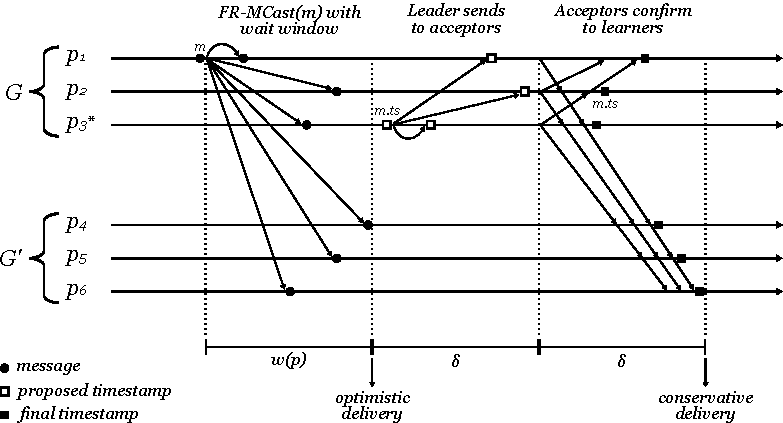
\includegraphics[width=0.8\linewidth]{images/paxos3d}
  \caption{Deciding the final timestamp and notifying all destination groups in three communication steps}
  \label{fig:paxosmanylearnergroups}
\end{figure}

\subsection{Optimistic Delivery}
\label{sec:optdel}

Even if a fifo reliable multicast primitive is used to send every message to each one of its destinations, guaranteeing its arrival in fifo order, messages from different senders may arrive in different orders at different destinations, so consensus is necessary to decide which order should be considered by all processes. However, we can predict the final delivery order using the initial timestamps assigned to the messages by their senders: if each process $p$ waits long enough before proposing some message $m$, every message $m' : m'.ts < m.ts$ will arrive eventually and $p$ will be able to propose them in the same order of their initial timestamps, achieving total order without needing any consensus for that.

The problem is then how to define the length of such wait window for each message $m$ such that every message prior to $m$ will have already been received when the window time has elapsed. As the message delay is unpredictable in asynchronous systems, we make an optimistic assumption:

\begin{center}
\emph{A2: every process $p$ knows a value $w(p)$, which is at least the maximum sum of the message delay bound plus the clock deviation between $p$ and any process $p'$ which could send a message to $p$.}
\end{center}

More formally, for $p$ in group $g$, we can define $w(p)$ as $max_{q \in sendersTo(g)}(\delta(p,q)+\epsilon(p,q))$, where $q$ is a process, $\delta(p,q)$ is the maximum time a message takes to go all the way from $p$ to $q$ and $\epsilon(p,q)$ is the difference between the clocks of $p$ and $q$\footnote{If this difference is less than zero, it means that the clock value in $q$ is higher than that in $p$, so $p$ actually has to wait less for messages from $q$, as they will have higher timestamps because of the clock deviation.}. The clock deviation is mentioned in this assumption because the timestamp of each message $m$ is assigned according to the local clock of its sender and we want that, once $m$ has been proposed, no message $m' : m'.ts < m.ts$ arrives afterwards. If our optimistic assumption considered only the message transmission delay, such property would not be guaranteed. However, the assumption may not hold, so deliveries made based on it have to be confirmed. There would be then two deliveries for each message: an optimistic one, done within one communication step, and a conservative one, based on consensus and barriers. 

The optimistic delivery works as follows: after a new message $m$ has been \rmdel{}ed at $p$, instead of proposing it, $p$ %inserts it into an $optPending$ set. Then, $p$ 
waits until its own wallclock has a value greater than $m.ts + w(p)$. At this moment, if \emph{A2} holds, then all messages that could possibly have an initial timestamp lower than $m$ have already been received by $p$. Therefore, such messages can be \optdel{}ed in the order of their initial timestamps.

If every process $q$ of $g$ has estimated $w(q)$ correctly, then all processes of $g$ will propose all messages from such group in the same order, which is that of the initial timestamps. If this happens, there will be no timestamp changes and the optimistic delivery will be correct. Not changing timestamps allows for further improvement: if barriers are being requested for each message $m$, as described in Section \ref{sec:nullondemand}, the barrier requests may be sent to $blockers(m)$ at the same time as $m$ is \rmcast{} by its sender.

If \emph{A2} fails to hold and some message $m$ is received by some process $p$ after a message $m'$ has been already \optdel{}ed by $p$, where $m.ts < m'.ts$, then the optimistic delivery algorithm has made a \textit{mistake}. Such mistake can be figured out by the application from the difference between the optimistic delivery order and the conservative one. The application should then correct whatever problems this mistake might have caused. Besides, when such a mistake happens, it means that the timestamp of a message may have changed and that a new barrier request may have to be sent to $blockers(m)$ once the new timestamp has been defined.

%The delivery time of each message $m$ will now depend on whether the assumption \emph{A2} holds or not while $m$ is being handled by the algorithm. If it does hold, it will be \optdel{}ed in the correct order within $w(p)$ and, as a barrier request was done in parallel with the conservative delivery algorithm, it will take $w(p) + 2\tconsm + \delta$ to \consdel{} $m$ in the worst case. If it does not hold, after $w(p)$, $m$ may be \optdel{}ed in an invalid order and, since its timestamp may have changed, a new barrier request may have to be done. Therefore, the worst case conservative message delivery time when the optimistic assumption does not hold and some message is delivered out of order would be $2w(p) + 4\tconsm + \delta$.

%Figure \ref{fig:optdel} illustrates both cases, when the optimistic assumption holds and otherwise. Three groups are shown: $G$, $G'$ and $G_b$, where $sendersTo(G) = \{G_b\}$, $sendersTo(G') = \{G\}$ and \mbox{$sendersTo(G_b) = \emptyset$}. A message $m : m.src = G \wedge m.dst = \{G, G'\}$ is \amcast{} and, at the same time, a barrier request is sent to the only group in $blockers(m)$, which is $G_b$. In (a), the optimistic assumption holds, so no message $m' : m'.ts < m.ts$ arrives after the proposal of $m$; in (b), however, it is necessary to make a second barrier request.

% \begin{figure} 
%   \centering
%   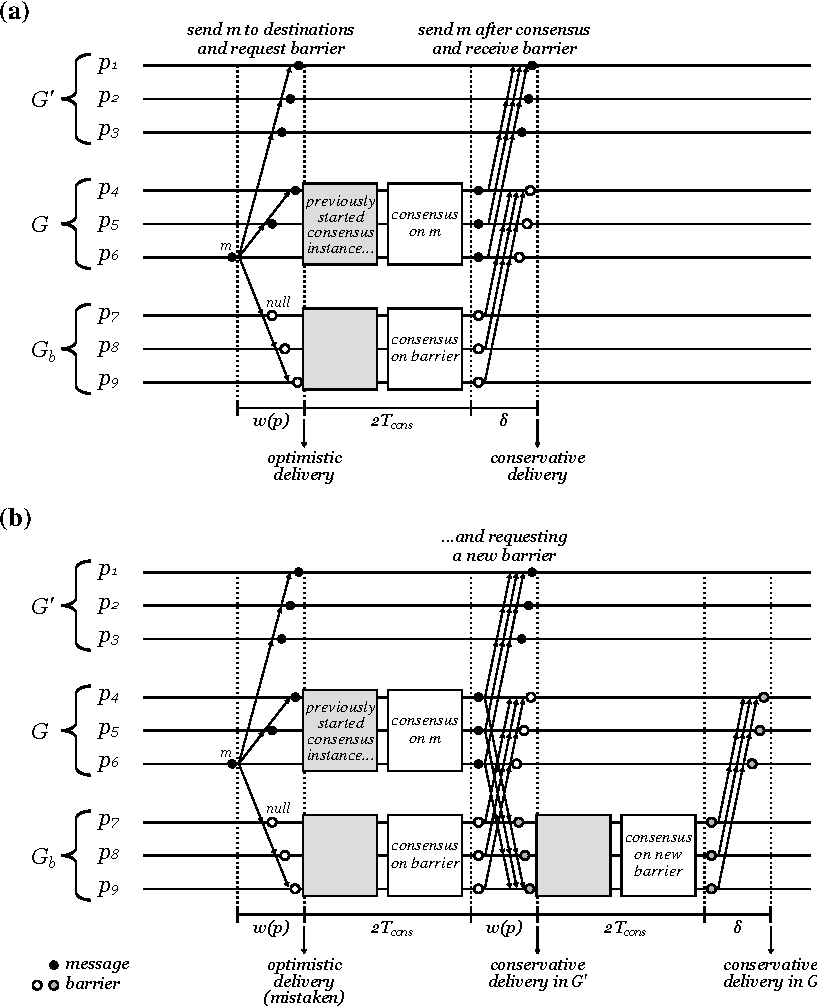
\includegraphics[width=0.8\linewidth]{images/optdel}
%   \caption{Execution examples when the optimistic assumption holds (a) and when it fails to hold (b)}
%   \label{fig:optdel}
% \end{figure}

% 
% \begin{algorithm}
% \begin{distribalgo}[1]
% 
% \blankline
% \INDENT {Initialization}
%   \STATE $k \leftarrow 0$, $nextProp \leftarrow 0$, $\decided \leftarrow \emptyset$, $\localmsgs \leftarrow \emptyset$, $optPending \leftarrow \emptyset$, $\stamped \leftarrow \emptyset$
%   \INDENT{\textbf{for all} $G' \in sendersTo(G)$ \textbf{do}}
%     \STATE $barrier(G',G) \leftarrow -\infty$ 
%   \ENDINDENT
% \ENDINDENT 
% 
% \blankline
% \INDENT{\textit{To send a message $m$} -- \amcastarg{m}}
%   \STATE $m.ts \leftarrow getTime()$  
%   \COMMENT{current wallclock value as the timestamp of $m$}
%   \STATE \rmcastarg{$m$}{$m.dst \cup \{G\} \cup blockers(m)$}
% %  \INDENT{\textbf{for all} $p' \in m.dst \cup \{G\} \cup blockers(m)$ \textbf{do}}
% %    \STATE send($p'$, $m$)    
% %    \COMMENT{send optimistically $m$ to all involved processes}
% %  \ENDINDENT
% \ENDINDENT
% 
% \blankline
% \INDENT{\textit{When} \rmdelarg{$m'$}}
%   \IF {$G \neq m'.src$ $\wedge$ $\exists G' \in (m'.dst \cap receiversFrom(G))$}
%     \STATE $null \leftarrow$ empty message
%     \STATE $null.src \leftarrow G$  \COMMENT{some other group needs a barrier from this one}
%     \STATE $null.ts \leftarrow m'.ts$ \label{algline:nulltsmts}
%     \STATE $null.dst \leftarrow m'.dst \cap receiversFrom(G)$
%     \STATE $optPending \leftarrow optPending \cup \{null\}$
%   \ENDIF
%   \IF {$m'.ts < getTime() - w(p) \vee G \notin m'.dst$}
%     \STATE discard $m'$
%     \COMMENT{late commands probably lead to out-of-order delivery}
%   \ELSE
%     \STATE $optPending \leftarrow optPending$ $\cup$ $\{m'\}$
%   \ENDIF
% \ENDINDENT
% 
% \blankline
% \INDENT{\textit{When $\exists m \in optPending : getTime() > m.ts + w(p)$ $\wedge\ \nexists m' \in optPending: m'.ts < m.ts$}}
%   \STATE $optPending \leftarrow optPending \setminus \{m\}$
%   \IF {$G \in m.dst \wedge m \neq null$}
%     \STATE \optdelarg{$m$}  
%   \ENDIF
%   \IF {$G = m.src$}
%     \STATE $\localmsgs \leftarrow \localmsgs \cup \{m\}$
%   \ENDIF
% \ENDINDENT
% 
% \blankline
% \INDENT{\textit{When $\exists m \in \localmsgs \wedge nextProp = k$}}
% %  \STATE $\localmsgs \leftarrow \localmsgs \setminus \{m\}$
% %  \IF {$m \notin \decided \wedge \nexists m' \in \decided: m'.ts > m.ts$}
%     \STATE $\localmsgs \leftarrow \localmsgs \setminus (\decided \cup \{m' : \exists m'' \in \decided \wedge m'.ts < m''.ts \wedge m' \neq null\})$ \label{algline:keepnull}
%     \IF {$\localmsgs \neq \emptyset$}
%       \STATE $nextProp \leftarrow k + 1$
%       \STATE propose$_g$($k$,$\localmsgs$)
%     \ENDIF
% %  \ENDIF
% \ENDINDENT
% 
% \blankline
% \INDENT{\textit{When} decide$_g$($k$,$msgSet$)}
% %  \STATE $m.gs \leftarrow k$
%   \STATE $\decided \leftarrow \decided \cup msgSet$
%   \INDENT{\textbf{for all} $m \in msgSet : G \in m.dst \wedge m \neq null$ \textbf{do}} \label{algline:checkcons}
%     \STATE $\stamped \leftarrow \stamped \cup \{m\}$
%   \ENDINDENT
%   \INDENT{\textbf{while} $\exists m \in msgSet : (\forall m' \in msgSet : m \neq m' \Rightarrow m.ts < m'.ts)$ \textbf{do}}
%     \INDENT{\textbf{for all} $p' \in m.dst \setminus \{G\}$ \textbf{do}}
%       \STATE send($p'$, $\{m, \text{`cons'}\}$)
%       \COMMENT{this message is sent through a fifo lossless channel}
%     \ENDINDENT
%     \STATE $msgSet \leftarrow msgSet \setminus \{m\}$
%     \COMMENT{the messages are sent in ascending order of timestamp}
%   \ENDINDENT
%   \STATE $nextProp \leftarrow k + 1$
%   \STATE $k \leftarrow k + 1$  
% \ENDINDENT
% 
% \blankline
% \INDENT{\textit{When} receive($\{m',\{\text{`cons'}\}$)}  
%   \IF {$m' \notin\ \stamped \wedge m' \notin\ \delivered \wedge m' \neq\ null$}
%     \STATE $\stamped \leftarrow \stamped \cup \{m\}$
%   \ENDIF
%   \STATE $barrier(m'.src,G) \leftarrow max(m'.ts, barrier(m'.src,G))$  \COMMENT{channels are fifo, but there are different senders}
% \ENDINDENT
% 
% \blankline
% \INDENT{\textit{When $\exists m \in \stamped : \forall G' \in sendersTo(G): m.ts < barrier(G',G)$\\ $\wedge\ \nexists m' \in \stamped : m'.ts < m.ts$ }}
%   \STATE $\stamped \leftarrow \stamped \setminus \{m\}$
%   \STATE \consdelarg{$m$}
%   \STATE $\delivered \leftarrow \delivered \cup \{m\}$
% 
% \blankline
% \ENDINDENT
% 
% \caption{\amcastarg{m} -- executed by every process $p$ from group $G$}
% \label{algorithm:nullondemand}
% \end{distribalgo}
% \end{algorithm}

\subsection{Timestamp composition}
\label{sec:compositets}

\textit{\textbf{I'm not sure of how good this `optimization' is; maybe it's not worth putting on the paper...}}

Barrier requests for each message $m$ may be sent before $m$'s final timestamp is decided. However, if $m.ts$ changes, new barrier requests will probably be deemed necessary. For instance, let $m$ and $m'$ be two messages sent by different processes of the same group $g$, where their initial timestamps are such that $m.ts < m'.ts$. Assume also that barrier requests have been sent at the same time as such messages were being sent. Suppose that some process $p$ from $g$, due to some asynchronous behavior of the system, received $m'$ first, proposed it and had $m'$ decided before $m$. As $m$ will be decided afterwards, its timestamp will be made greater than that of $m'$. Therefore, the barriers requested in order to deliver $m$ might not suffice anymore, requiring new, higher ones.

An approach to reduce this problem could be by using composite timestamps. Instead of relying on a single value -- apart from the message id for breaking ties --, two values could be used: one related to the instant when the message was created and one sequence number incremented only when the timestamp should be increased. The former we call $rtc$, standing for real-time clock, and the latter we call $seq$. Being $m$ any message, $m.ts = (rtc,seq)$. The second value is used only to break ties when the first one is equal between some two messages. In the case when the timestamp of $m$ has to be made greater than that of some message $m'$, where $m'.ts = (rtc', seq')$, the timestamp of $m$ would be changed to $(rtc', seq'+1)$.

In reply to the barrier request for some message $m : m.ts = (rtc,seq)$, a process in $blockers(m)$ would enqueue some message $b : b.ts = (rtc + 1, \text{---})$ to be sent to $m.src$. The whole purpose of this is: if two messages $m$ and $m'$, with initial timestamps $m.ts < m'.ts$ had barriers requested at the same time as their creation, even if $m.ts$ is changed because of $m'$, the barrier received for the delivery of $m'$ will probably also serve $m$ -- except when \mbox{$blockers(m) \setminus blockers(m') \neq \emptyset$} or when an empty message is enqueued, since no barrier is requested for empty messages, but they can still cause timestamp changes in other messages

\subsection{Relaxing validity and discarding stale messages}
\label{sec:discard}

When employing the optimistic delivery proposed in Section \ref{sec:optdel}, some messages may still need to have their initial timestamp changed as a possible consequence of the optimistic assumption \emph{A2} not holding. Thus it may be necessary to request new, higher barrier values, resulting in longer delivery latencies, not only for the messages whose timestamp changed, but also for those after them in the delivery queue. Besides, delivering messages out of the initial timestamp order may increase the number of mistakes made by the optimistic delivery. A simple way to eliminate the possibility of having to change timestamps is by discarding messages that arrived too late, that is, with a timestamp lower than that of some already delivered message.

Although discarding messages which do not follow the initial timestamp order conflicts with the properties we have defined for the \amcast{} primitive, we describe this approach here because it brings the benefit of decreased number of mistakes and lower message delivery latency. The validity property would have to be changed to:

\begin{itemize}
  \item[(i)] If a correct process $p$ \amcast{}s $m$ and the optimistic assumption \emph{A2} holds, then  every correct process $q \in m.dst$ \amdel{}s $m$ \emph{(optimistic uniform validity)}.
\end{itemize}

%\textbf{Optimistic Uniform Validity}: If a process \amcast{}s $m$ and the optimistic assumption \emph{A2} holds, then one of the correct processes that is a destination of $m$ eventually \consdel{}s $m$.

The problem with changing the original uniform validity property is that it could make the multicast primitive impracticable for some applications. Nevertheless, some other applications not only do not require messages to be delivered if they arrive out of order, but also it is better not to deliver such messages at all -- such as real-time streams of audio or video or online real-time multiplayer games. In any case, the application could specify whether each message might be discarded or not.





\subsection{Complexity analysis}
\label{sec:complexity}

In this section, we analyse the time complexity of our atomic multicast protocol. We consider an optimized version of the algorithm described in Section \ref{sec:baseline}, that is, we are assuming that the optimizations suggested in Section \ref{sec:optimized} have been implemented. Therefore, our time complexity analysis considers that:

\begin{itemize}
  \item before proposing some message $m$, any process $p$ which proposes it waits for $w(p)$ time, after which $m$ can also be \optdel{}ed;
  \item consensus instances are run in parallel;
  \item consensus is implemented with Paxos and one of the processes of each group is elected as leader;
  \item when a process $p$ is \amcast{}ing some message $m$, before \rmcast{}ing it to the other processes of $group(p)$, $p$ sends barrier requests to all processes in $blockers(m)$;
  \item given any message $m$, when some process $p$ from $m.src$ know thats $m.ts$ has changed and that higher barrier values must be requested, $p$ sends such barrier requests.
\end{itemize}





%===                               ================
%===     PROOFS OF CORRECTNESS     ================
%===                               ================     

\section{Proof of correctness}
\label{sec:proofs}

Here, we prove that the \amcast{} primitive ensures the properties defined in section \ref{sec:model} -- uniform validity, uniform agreement, uniform integrity, uniform total order and fifo order. To do this, we prove that \mbox{Algorithm \ref{algorithm:deliveryminimal}}, when used along with \mbox{Algorithm \ref{algorithm:nullperiodic}}, ensures these properties. Although there are different processes executing such algorithms at the same time, we assume that there is no concurrency on the execution of the algorithms in any single process.





\subsection{Uniform Validity}




%===           ====================================
%===   LEMMA   ====================================
%===           ====================================
\begin{lems} \label{lemma:mcastdecided}
Once every correct process in a group $g$ has inserted a message $m$ into $\localmsgs$, $m$ will eventually be decided by all correct processes of $g$.
\end{lems}

\begin{proof}
In Algorithm \ref{algorithm:deliveryminimal}, once each correct process $p$ from $g$ has received $m$ and inserted into its $\localmsgs$ set, $m$ will be proposed by $p$ in every consensus instance, until $m$ has been inserted into $\decided$ (lines \ref{algline:undecided} and \ref{algline:propose}). As $m$ is inserted into $\decided$ only after being decided (l. \ref{algline:addtodecided}), every correct processes of $g$ will propose $m$ at some point, so $m$ will eventually be decided. From the uniform agreement property of consensus, as $m$ is decided, all correct processes of $g$ decide $m$.
\end{proof}







%===           ====================================
%===   LEMMA   ====================================
%===           ====================================
\begin{lems} \label{lemma:mcastbarpending}
Once a message $m$ has been \amcast{}, it will be inserted into the $\stamped$ set of all the correct processes to which such message has been addressed.
\end{lems}

\begin{proof}
In Algorithm \ref{algorithm:deliveryminimal}, whenever a process in a group $g$ \amcast{}s a message, it is first \rmcast{} to all processes in $g$ (l. \ref{algline:rmlocal}). From the properties of the \rmcast{} primitive, every correct process from $g$ \rmdel{}s $m$ and inserts it into $\localmsgs$ (l. \ref{algline:addtogroupmsgs}). From Lemma \ref{lemma:mcastdecided}, $m$ will eventually be decided within $g$. When this happens, if $g \in m.dst$, every correct process of $g$ also inserts $m$ into $\stamped$ (l. \ref{algline:insbp2}). Besides, each correct process in $g$ \rmcast{}s $m$ to all other groups that $m$ is adressed to (l. \ref{algline:rmothers}).

Let $q$ be any correct process in a destination group $h$ of the message $m$, such that $h \neq g$. From the properties of \rmcast{}, $q$ will \rmdel{} $m$. Once $m$ is \rmdel{}ed by $q$, such message is inserted into the $\stamped$ set of $q$, unless this has been already done (lines \ref{algline:notbptwice} and \ref{algline:insbp1}).
\end{proof}



%===           ====================================
%===   LEMMA   ====================================
%===           ====================================
\begin{lems} \label{lemma:barrierperiodic}
  Given a correct process $p$ and a message $m$, $p$ eventually receives some message $m' : m'.ts > m.ts$ from every group in $sendersTo(gropu(p))$.% and insert it into its $stamped$ set.
\end{lems}

\begin{proof}Let $g = group(p)$ and let $h$ be any group in $sendersTo(g)$. Every process $q \in h$ executes Algorithm \ref{algorithm:nullperiodic}, inserting messages with ever-increasing timestamp values into $\localmsgs$. Therefore, at some point, every process from $h$ will propose some message $m' : m'.ts > m.ts$. As one of these proposals will be decided, then one of these messages will be \rmcast{} to $g$. From the properties of \rmcast, $g$ will deliver it.
%
%which means that, from Lemma \ref{lemma:mcastdecided}
% 
% 
% thus inserting messages with ever-increasing timestamp values to all other groups that might receive a message from $h$, i.e., to every process $r$, such that $\exists i \in \Gamma: h \in sendersTo(i) \wedge r \in i$. %Also, if $G \in receiversFrom(G')$, then $G' \in sendersTo(G)$. 
% Therefore, at some point, all correct processes of each group $h$ in $sendersTo(g)$ will have inserted a message $m'$ -- be it $null$ or not -- with a timestamp greater than or equal to that of $m$ into their respective $\localmsgs$ lists (l. \ref{algline:enqnull} of Algorithm \ref{algorithm:nullperiodic}). From Lemma \ref{lemma:mcastdecided}, all processes of $h$ will decide $m'$ and \rmcast{} it to $g$. From the properties of the \rmcast{} primitive, $p$ will \rmdel{} $m'$ and insert it into its $\stamped$ set (l. \ref{algline:insbp1} of Algorithm \ref{algorithm:deliveryminimal}). From the algorithm, the timestamps of the messages no longer change after being inserted into $\stamped$ so, eventually, $p$ will have in such set a barrier with a value greater than or equal to $m.ts$ from each group in $sendersTo(g)$.
\end{proof}







%===           ====================================
%===   LEMMA   ====================================
%===           ====================================
\begin{lems} \label{lemma:lowertsfrmcastfirst}
Given any two messages $m$ and $m'$ sent from the same group $g$, if a process $p \in g$ decides that their final timestamps are such that $m.ts < m'.ts$, then $p$ does not \rmcast{} $m'$ before $m$.
\end{lems}

\begin{proof}
Assume, by way of contradiction, that $p$ \rmcast{}s $m'$ first. This means that $m'$ was inserted into $\decided$ first. When $m$ is handled in the algorithm (lines \ref{algline:decidedloopbegin} to \ref{algline:rmothers}), $m'$ is already there. Then, $p$ decides that the final timestamp of $m$ is $m.ts > m'.ts$ (lines \ref{algline:decidedloopbegin} to \ref{algline:changetsafterdecision}), which is a contradiction.
\end{proof}





%===           ====================================
%===   LEMMA   ====================================
%===           ====================================
\begin{lems} \label{lemma:agreetimestamps}
Given any two correct processes and a message $m$, if each of such processes is either a destination of $m$ or belongs to $m.src$, then such processes agree on the final timestamp of $m$.
\end{lems}

\begin{proof}
Let $p$, from group $g$, be the process that is \amcast{}ing $m$. We can prove this lemma by demonstrating that any other process $q \in g \cup m.dst$ will agree with $p$ on the timestamp of $m$. Let us first consider the case where $q$ also belongs to $g$. The proof for this case can be done by induction on the identifier $k$ of each consensus instance within $g$:\\

\noindent Base case ($k=1$): As this is the first consensus instance within $g$, it means that $\decided$ was empty when such instance started. From the agreement property of consensus, we know that $p$ and $q$ decide the same contents for $msgSet$ \mbox{(l. \ref{algline:decide})}. Each message included in such agreed set also includes an initial timestamp field. As the $\decided$ set is empty, such timestamps are not changed in neither $p$ or $q$ (lines \ref{algline:decidedloopbegin} to \ref{algline:changetsafterdecision}). Therefore, both processes consider the same timestamp value for every message. Besides, as the $msgSet$ is the same for both, the $\decided$ set remains identical in $p$ and $q$.\\

\noindent Induction step: Suppose that $p$ and $q$ have already learnt the decisions of instance $k$, their $\decided$ sets remained identical and they decided the same timestamp value for each message sent from some process in their group so far. From the algorithm, all processes within a group learn all decisions in the same order, which is that of the consensus instance identifiers. Therefore, both $p$ and $q$ will next learn the decision of the instance $k+1$. From the agreement property of consensus, the $msgSet$ decided is the same for both processes. In the Algorithm \ref{algorithm:deliveryminimal}, the timestamps may be changed after the consensus decision only in line \ref{algline:changetsafterdecision}, based on what is already in the $\decided$ set (lines \ref{algline:decidedloopbegin} to \ref{algline:changetsafterdecision}). As the $msgSet$ and $\decided$ sets are each identical in $p$ and $q$, they will make the exact same change to the timestamp of each message in the \textit{while} loop (lines \ref{algline:decidedloopbegin} to \ref{algline:rmothers}). Therefore, they also agree on the timestamps of each message decided on consensus instance $k+1$ and their $\decided$ sets remain identical.\\

Now, regarding the case of $q$ not belonging to $g$, let $r$ be any correct process of such group. After setting the final timestamp of $m$ (l. \ref{algline:decidedloopbegin} to l. \ref{algline:rmothers}), $r$ \rmcast{}s $m$ to $group(q)$ (l. \ref{algline:rmothers}). From the algorithm, after \rmdel{}ing $m$, $q$ never changes the value of $m.ts$, set by $q$ in accordance with $p$.% As any two processes on the same group from which $m$ has been multicast agree on its timestamp, and since any process from other group which is also a destination of $m$ agree on its timestamp as well, than any two processes that are destinations of $m$ agree on its timestamp.
\end{proof}






%===           ====================================
%===   LEMMA   ====================================
%===           ====================================
\begin{lems} \label{lemma:groupfifo}
If a process $p$ from a group $g$ has received a message $m$ from another group $h \neq g$, then $p$ has also received from $h$ any message $m' : m'.ts < m.ts$.
\end{lems}

\begin{proof}
In Algorithm \ref{algorithm:deliveryminimal}, every process $q$ from $h$ sends messages to the processes of $g$, including $p$, using a fifo channel, via the \rmcast{} primitive. From the properties of consensus, we know that all correct processes from $h$ will decide the same messages in each consensus instance $k$. From Lemma \ref{lemma:lowertsfrmcastfirst} and Lemma \ref{lemma:agreetimestamps}, every correct process from $h$ \rmcast{}s to $g$ every message $m : m.src = h \wedge g \in m.dst$ (l. \ref{algline:rmothers} of Algorithm \ref{algorithm:deliveryminimal}) in the same order, which is that of the timestamps. From the fifo property of \rmcast{}, we know that $p$ will \rmdel{} all of such messages from each process of $h$ in ascending order of timestamps. Although such messages will arrive from different senders and may be out of order at $p$, once $p$ received some message $m$ from some process of $h$, $p$ has also received any message \mbox{$m' : m'.src = h \wedge g \in m.dst\wedge m'.ts < m.ts$}.
%
%Assume, by way of contradiction, that $p$ received a message $m' : m'.ts < m.ts$ from some process $r \in h$ after having received $m$ from $q$. As $m'.src = m.src$ and $q$ \rmcast{}s to $g$ every message $m : m.src = h \wedge g \in m.dst$, this means that $q$ will send $m'$ afterwards, contradicting the fact that the processes in $h$ agree on each batch of messages decided and send them to $g$ in the same fifo order.
\end{proof}






%===           ====================================
%===   LEMMA   ====================================
%===           ====================================
% \begin{lems} \label{lemma:alwaysbpdel}
% Once a message has been inserted into the $\localmsgs$ set of a given process, it will always belong to it.
% \end{lems}
% 
% \begin{proof}
% Immediate from the algorithm, considering that a message is never removed from the $\localmsgs$.
% \end{proof}




%===           ====================================
%===   LEMMA   ====================================
%===           ====================================
\begin{lems} \label{lemma:oncedecidednotsmaller}
Once a process $p$ has inserted a message $m$ into its $\stamped$ set, no message $m' : m'.ts < m.ts$ from $m.src$ will be inserted into such $\stamped$ set afterwards.
\end{lems}

\begin{proof}
Let $g$ be the group of $p$. Group $g$ is either $m.src$ or not. In the former case, before inserting any message $m' : m'.src = m.src$ into $\stamped$, $p$ has to decide $m'$ first. When a message is decided by $p$, $p$ checks whether some other message which was decided previously has a timestamp lower than $m'$ and, if that is the case, the timestamp of $m'$ is changed to a value greater than that of any other message already decided (lines \ref{algline:decidedloopbegin} to \ref{algline:changetsafterdecision} of Algorithm \ref{algorithm:deliveryminimal}). Only then $m'$ may be inserted into the $\stamped$ set of $p$ (l. \ref{algline:insbp2}). Therefore, $p$ inserts messages from other processes of $g$ into its $\stamped$ set in ascending order of timestamps. Besides, the messages from $g$ are \rmcast{} to other groups in this same order (l. \ref{algline:rmothers}) by all correct processes of $g$, from the uniform agreement property of consensus.

In the case where $g \neq m.src$, $p$ inserts $m$ into $\stamped$ in line \ref{algline:insbp1}. Considering that when $p$ receives any message from $m.src$, any other other message from $m.src$ with a lower timestamp has already been received (from Lemma \ref{lemma:groupfifo}), we can infer that, once $p$ inserts $m$ into $\stamped$, no message $m' : m'.ts < m.ts$ from $m.src$ will be inserted into the the $\stamped$ set of $p$ afterwards.
\end{proof}





%===           ====================================
%===   LEMMA   ====================================
%===           ====================================
\begin{lems} \label{lemma:oncebpwilldel}
Once a message $m \neq null$ has been inserted into the $\stamped$ set of a correct process $p$, $m$ is eventually delivered by $p$.
\end{lems}

\begin{proof}
Let $g = group(p)$. Eventually, $p$ will have received, from every group in $sendersTo(g)$, some message with a timestamp greater than $m.ts$ (from Lemma \ref{lemma:barrierperiodic}). Once this happens, no more messages with a timestamp lower than that of $m$ will be inserted into the $\stamped$ set of $p$ (from Lemma \ref{lemma:oncedecidednotsmaller} and the definition of $sendersTo(g)$). Let $ready$ be the set of $m$ plus all undelivered messages from $\stamped$ whose timestamps are lower than that of $m$, that is, $ready = \{m\} \cup \{m' : m' \in \stamped \setminus \delivered \wedge m'.ts < m.ts\}$.

We can infer that no more messages will be included in this set, meaning that any other message that might be later inserted into $\stamped$ will have a timestamp greater than that of any message in $ready$. Besides, the barriers received apply to all messages in this set, since their timestamps are not greater than $m.ts$. Each one of these messages will eventually be inserted into $\delivered$ and, if it is different from $null$, it will be delivered by $p$. We prove this by induction on the position $i$ of each message $m_i$ in $ready$, in ascending order of timestamps.\\
\\
\noindent Base case ($i=1$): Let $m_1$ be the first message in $ready$, i.e., \mbox{$\nexists m \in \stamped \setminus \delivered : m.ts < m_1.ts$}. We know that all the necessary barriers have been received already, so $m_1$ satisfies all conditions from lines \ref{algline:condel1} and \ref{algline:condel2} of \mbox{Algorithm \ref{algorithm:deliveryminimal}}. Therefore, $m_1$ will be inserted into $\delivered$, after which $m_1$ will no longer belong to $\stamped \setminus \delivered$. Also, if $m_1 \neq null$, $m_1$ will be delivered.\\
\\
\noindent Induction step: Suppose that $m_{i}$ will eventually be inserted into the $\delivered$ set. Once this happens, it means that $m_{i}$ was the first message in $\stamped \setminus \delivered$ in ascending timestamp order. Since no more messages have been inserted into $ready$, as soon as $m_{i}$ is inserted into $\delivered$, $m_{i+1}$ will be the first one in $\stamped \setminus \delivered$, having, therefore, the lowest timestamp in such set. Then, as all barriers necessary for $m$ have already been received and $m_{i+1}.ts \leq m.ts$, $m$ will satisfy both conditions of lines \ref{algline:condel1} and \ref{algline:condel2} of \mbox{Algorithm \ref{algorithm:deliveryminimal}}. Thus, $m_{i+1}$ will also be inserted into the $\delivered$ set and, if $m_{i+1} \neq null$, it will be delivered.
\end{proof}


%===                 ==============================
%===   PROPOSITION   ==============================
%===                 ==============================
\begin{props} \label{props:validity}
Once a process \amcast{}s a message, then all correct processes that are destinations of that message eventually deliver it.
\end{props}

\begin{proof}
Immediate from Lemma \ref{lemma:mcastbarpending} and Lemma \ref{lemma:oncebpwilldel}.%Immediate from Lemma \ref{lemma:mcastbarpending}, Lemma \ref{lemma:oncebpwilldel}, and from the assumption that the application will not \amcast{} a $null$ message -- not in the \amcast{} protocol level at least; if the application needs to \amcast{} an empty message, in the protocol level it would not be handled as a $null$ message.
\end{proof}





\subsection{Uniform Integrity}





%===                 ==============================
%===   PROPOSITION   ==============================
%===                 ==============================
\begin{props} \label{props:integrity}
If a message $m$ was delivered by some process $p$ of group $g$, then (1) $m$ has been \amcast{} before, (2) $g \in m.dst$ and (3) it has not been \amdel{}ed by $p$ before.
\end{props}

\begin{proof}
From lines \ref{algline:condel1} to \ref{algline:addtodelivered} of Algorithm \ref{algorithm:deliveryminimal}, and since no message is removed from $\delivered$, no message can be delivered twice, satisfying (3). For a message $m$ to be \amdel{}ed (l. \ref{algline:consdeliver}), it must belong to the $\stamped$ set (l. \ref{algline:condel1}).  There are two possibilities to when $m$ has been inserted into such set:
\begin{itemize}
  \item $m$ has been originated in the same same group of $p$, that is, $p \in m.src$, which means that $m$ was inserted into $\stamped$ in line \ref{algline:insbp2} of Algorithm \ref{algorithm:deliveryminimal}, or
  \item $m$ has been sent from a group $h \neq g$, which means that it was inserted by $p$ into $\stamped$ in line \ref{algline:insbp1}. 
\end{itemize}

For the case when $p \in m.src$, $m$ can be inserted into $\stamped$ only in line \ref{algline:insbp2}, which means that $g \in m.dst$, satisfying condition (2) for this case. Also, this happens only when $m$ has been decided in some consensus instance within $g$. To have been decided within $g$, from the properties of consensus, we know that it must have been proposed by some process of $g$, which happens in line \ref{algline:propose}. In line \ref{algline:propose}, for a message to be proposed, it must be in $\localmsgs \setminus \decided$, as the contents of such set are the value proposed. For a message to be in $\localmsgs$, it must have been inserted there, which happens only in line \ref{algline:addtogroupmsgs}. For l. \ref{algline:addtogroupmsgs} to be executed, $m$ must have been \rmdel{}ed and $g$ must be the source group of $m$, that is, $g = m.src$. For a message to be \rmcast{} by a process to its own group, a \amcastarg{$m$} call must have been made -- which satisfies condition (1) --, for line \ref{algline:rmlocal} is the only one where a process \rmcast{}s a message to its own group. 

As for the case when $p \notin m.src$, $m$ is inserted into the $stamped$ set of process $p$ in line \ref{algline:insbp1}, when it has been \rmdel{}ed. For a process $q \in h$, where $h = m.src$, to \rmcast{} $m$, $m$ must have been decided within $h$, which means that it was proposed within $h$. Therefore it was \amcast{} -- satisfying condition (1) -- by $h$ to $g$. From line \ref{algline:rmothers}, $g$ necessarily belongs to $m.dst$, satisfying condition (2).

Finally, as for Algorithm \ref{algorithm:nullperiodic}, $null$ messages are never delivered, so they will never violate the uniform integrity property.
\end{proof}






\subsection{Uniform Agreement}

%===                 ==============================
%===   PROPOSITION   ==============================
%===                 ==============================
\begin{props} \label{props:agreement}
If a correct process which is a destination of a message $m$ delivers it, then all correct processes that are also destinations of $m$ deliver it as well.
\end{props}

\begin{proof}
Immediate from Proposition \ref{props:validity} and Proposition \ref{props:integrity}.
\end{proof}






\subsection{Atomic Order}






%===           ====================================
%===   LEMMA   ====================================
%===           ====================================
\begin{lems} \label{lemma:respecttimestamps}
If two messages $m$ and $m'$, both different from $null$, have a correct process $p$ as a destination, and $m.ts < m'.ts$, then $p$ \amdel{}s $m'$ after \amdel{}ing $m$.
\end{lems}

\begin{proof}
Suppose, by way of contradiction, that $m'$ is delivered by $p$ before $m$. Message $m$ either has already been inserted into $\stamped$ or not. In the former case, as $m \neq null$ and $m$ has not been delivered, then $m$ belongs to $\stamped \setminus \delivered$. Therefore, $m'$ could not have been delivered, since $m.ts < m'.ts$ and it would not satisfy the condition from line \ref{algline:condel1} until $m$ has been delivered, so we have a contradiction in the case where $m$ was already in $\stamped$.

The other case is when $m$ has not been inserted into $\stamped$. From line \ref{algline:condel2} of Algorithm \ref{algorithm:deliveryminimal}, and since $m'$ has been delivered, we know that $p$ has received some barrier $b > m'.ts$ from every group in $sendersTo(group(p))$. Therefore, from Lemma \ref{lemma:oncedecidednotsmaller}, and since any barrier is also a message, we know that any new message that arrives at $p$ will have a timestamp greater than $m'.ts$. As $m$ has arrived after $m'$, then $m.ts > m'.ts$, which is also a contradiction.

We have proven that the timestamp order will not be violated by $p$. Considering that, once a message has been multicast, it will be delivered (Proposition \ref{props:validity}), then we know that all messages will be delivered by $p$, and in the correct timestamp order.\end{proof}




%===                 ==============================
%===   PROPOSITION   ==============================
%===                 ==============================
\begin{props} \label{props:atomicorder}
If processes $p$ and $p'$ are both in $m.dst$ and $m'.dst$, then $p$ delivers $m$ before $m'$ if, and only if, $p'$ delivers $m$ before $m'$.
\end{props}

\begin{proof}
Immediate from Lemma \ref{lemma:agreetimestamps}, Lemma \ref{lemma:respecttimestamps} and Proposition \ref{props:agreement}.
\end{proof}



\subsection{Fifo Order}





%===           ====================================
%===   LEMMA   ====================================
%===           ====================================
\begin{lems} \label{lemma:fifofinalts}
If a process $p$, from group $g$, \amcast{}s $m'$ after $m$, then the final values of their timestamps will be such that $m.ts < m'.ts$.
\end{lems}

\begin{proof}
As both messages are sent from $g$, they have to be decided withing $g$. If $m$ and $m'$ are decided in different consensus instances, and $m$ is decided first, then, from lines \ref{algline:decidedloopbegin} to \ref{algline:changetsafterdecision}, $m'$ will necessarily have a timestamp greater than that of $m$. Therefore, the two possible ways of having $m'.ts < m.ts$ are: either $m'$ is decided before $m$, or both are decided in the same consensus instance, but the timestamp of $m$ is set to a value higher than that of $m'$.

From lines \ref{algline:gettime} and \ref{algline:rmlocal}, and the properties of \rmcast{}, we know that all correct processes of $g$ \rmdel{} $m$, then $m'$, which means that each process $q$ from $g$ also inserts them into its $\localmsgs$ set in this same order. Suppose, by way of contradiction, that $m'$ is decided before $m$. This implies that some process $q \in g$ proposed a message set that included $m'$, but not $m$. As $q$ inserted $m$ before $m'$ into $\localmsgs$, then $m$ had already been inserted by $q$ into $\decided$. This means that $m$ has been decided previously, which is a contradiction. Therefore, $m'$ is not decided before $m$.

As for the case where $m$ and $m'$ are decided in the same consensus instance, we know, from line \ref{algline:gettime}, that the initial timestamp of $m$ is already smaller than that of $m'$. Therefore, from line \ref{algline:decidedloopbegin}, $m$ is inserted into $\decided$ first. Even if the timestamp of $m$ has changed, as $m$ was already in $\decided$ before $m'$, we know that the final timestamp of $m'$ will again be made greater than that of $m$ (from lines \ref{algline:decidedloopbegin} to \ref{algline:changetsafterdecision}).
\end{proof}






%===                 ==============================
%===   PROPOSITION   ==============================
%===                 ==============================
\begin{props} \label{props:fifoorder}
If a process $p$ \amcast{}s $m$ before \amcast{}ing $m'$, then no process $q \in m.dst \cap m'.dst$ \amdel{}s $m'$ before delivering $m$.
\end{props}

\begin{proof}
Immediate from Lemma \ref{lemma:respecttimestamps} and Lemma \ref{lemma:fifofinalts}.
\end{proof}

\section{Related work}

\cite{sousa2002oto}: optimistic total order bcast in wans: for the opt-delivery to work properly, requires that the delay between each pair of processes stay constant (ours only requires that it never goes beyond $w(p)$ for each process $p$\ldots). sequencer based (no tolerance for failures of the sequencer). not mentioning multicast.

\section{Experimental results}

\section{Conclusion}

%\bibliographystyle{latex8}
%\bibliography{main}
\bibliographystyle{acm}
\bibliography{gftommog}
\end{document}

